
% CHAPTER 2

\chapter{METHODOLOGY}
\label{chp:Methodology}


\section{Methodology}

In this thesis work, the problem of dynamical formation control of heterogenous mobile robots is reduced down to two subproblems as local positioning system design and formation control system design. Local positioning subsystem proposes  a  solution for the localization of the agents in the environment with the low sensor capabilities. This part of the solution provides a basis for the formation control problem with the true state vectors of agents composed with the translational positions and velocities. Formation control subsystem proposes a solution to achieve desired complex shapes with heterogenous agents in the swarm.  In this chapter, details of the solution for these subproblems are presented in details. 

\begin{figure}[H]
	\caption{Flowchart of the Provided Solution}
	\centering
	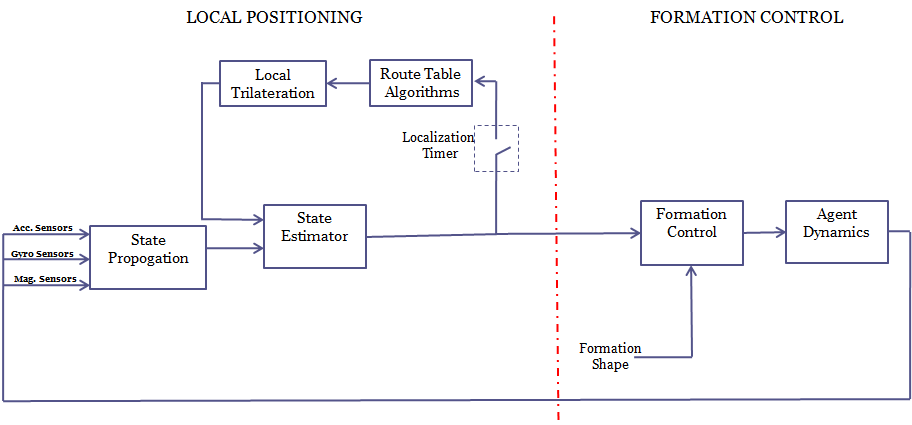
\includegraphics[scale = 0.65]{general_scheme}
\end{figure}


\subsection{Local Positioning System}

Local positioning system is a subsystem to provide a complete solution to the localization of the agents in the environment. As discussed in Section-xx(Objectives) , agents are expected to have low sensor capabilities and only a limited number of them have external position measurement sensors on their boards. The rest of the swarm have to maintain their position$\&$velocity data with the help of their inertial measurements. Propogation of the states with this type of measurements are always inclined to drift problems due to the errors$\&$noise and bias problems of the sensors and the state vectors composed with the translational positions and velocities have to be corrected with an external measurement. A complete solution for this type of problem is proposed in Figure-xx. 



\begin{figure}[H]
	\caption{Local Positioning System}
	\centering
	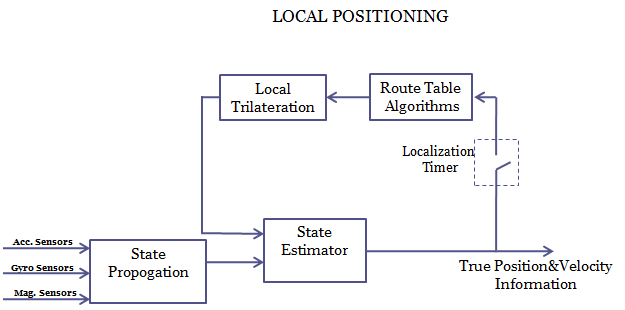
\includegraphics[scale = 0.65]{lps}
\end{figure}


As illustrated in Figure-xx, agents are expected to propogate their states with the help of acceleration, gyroscope and magnetometer sensors. Since the trilateration and route table determination processes require iterative and time consuming algorithms, a localization timer with a suitable period is implemented to the solution. Agents will correct their state vectors with the localization period of 3 seconds by measuring their positions with trilateration process and execute the update procedure in their state estimator algorithms. 



\subsubsection{Trilateration Process}

Trilateration process helps the agents to localize themselves with the help of their local neighbors.  Trilateration calculations use distance measurements to the nodes with known positions, to determine the coordinates of unknown positions[22]. These measurements are assumed to be done with the help of low cost range sensors like ultrasonic sensors.  Solution of the unknown position with the help of these distance measurements can be reduced down to a $A\vec{x} = \vec{b}$ type equation with the help of mathematical manipulations. The agents which has position sensors on their boards are called position beacons. Figure-xx illustrates a sample environment which consist of $i$ beacons and an agent which tries to localize itself with the help of distance measurements $r_i$ and the position data $B_i$ of the beacon nodes.
\begin{figure}[H]
	\caption{Environment for Trilateration Process}
	\centering
	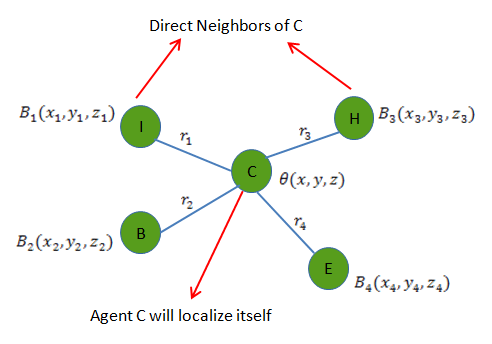
\includegraphics[scale = 0.65]{beacons}
\end{figure}

The distance function $\hat{r_i}$ can be written as follows;
\begin{equation} % eq 2
\hat{r_i} = \sqrt{(x-x_i)^2 + (y-y_i)^2+ (z-z_i)^2}    \hspace{0.3cm}   (i=1,2,...,n)
\end{equation}
where $i$ denotes the beacon number and $n$ is the total number of beacons. We have $n$ number of constraints in the solution of the localization problem. In our work, we have implemented a two dimensional localization solution with the assumption of each agent in the swarm have the same vertical position in Earth centered coordinate system. With this assumption, the problem for the localization process can be reduced down to a $A.\vec{x} =\vec{b} $ type linear system problem and the constraints will be circle functions rather than spherical ones, presented with

\begin{equation}
  (x-x_i)^2 + (y - y_i)^2 = {r_i}^2
\end{equation}

Lets assume $\theta = (x,y)$ is representing the coordinates of an agent which is trying to localize itself, and $B_1 = (x_1,y_1) ; B_2 = (x_2,y_2) ; B_3 = (x_3,y_3) ; ...  ; B_i = (x_i,y_i)$ are the agents with exactly known positions. 



If any of the beacons is considered as the reference beacon and named with an index of $r$, the distance equations can be provided as following 

The distance between the target agent and any beacon $i$
\begin{equation}
  d_i(\theta) = \sqrt{\left((x - x_i)^2 + (y - y_i)^2\right)}
\end{equation}

The distance between the referance beacon and the other beacons

\begin{equation}
d_ir(\theta) = \sqrt{\left((x_i - x_r)^2 + (y_i - y_r)^2\right)}
\end{equation}

The distance between the target agent and the referance beacon

\begin{equation}
d_r(\theta) = \sqrt{\left((x - x_r)^2 + (y - y_r)^2\right)}
\end{equation}

Adding and subtracting $x_j, y_j$ and $z_j$ in (6) gives

\begin{align*}
d_i^2(\theta) = & (x - x_r + x_r - x_i)^2 + (y - y_r + y_r - y_i)^2 \\
              = & (x - x_r)^2 + 2(x_r - x_i)(x - x_r) + (x_r-x_i)^2 \\ 
              + & (y - y_r)^2 + 2(y_r - y_i)(y - y_r) + (y_r - y_i)^2 \\               
\end{align*}


This equation yields to

\begin{align*}
 2((x_i - x_r)(x - x_r) + (y_i - y_r)(y - y_r)) = d_r^2(\theta) + d_{ir}^2 - d_i^2(\theta)
\end{align*}

this general statement is valid for each beacon with

\begin{align*}
  & (x_2 - x_1)(x - x_1) + (y_2 - y_1)(y - y_1) = \frac{1}{2} [d_r^2(\theta) + d_{2r}^2 - d_2^2(\theta)] \\
  & (x_3 - x_1)(x - x_1) + (y_3 - y_1)(y - y_1) = \frac{1}{2} [d_r^2(\theta) + d_{3r}^2 - d_3^2(\theta)] \\
  & ... \\
  & (x_n - x_1)(x - x_1) + (y_n - y_1)(y - y_1) = \frac{1}{2} [d_r^2(\theta) + d_{nr}^2 - d_n^2(\theta)] \\
\end{align*}

if $b_{ir}$ is defined for each beacon as follows:

\begin{equation}
  b_{ir} := \frac{1}{2}[d_r^2(\theta) + d_{ir}^2 - d_i^2(\theta)]
\end{equation}

then the linearized system equations can be represented with $A\vec{x} = \vec{b}$ type equation where;

\begin{equation}
			A = \begin{bmatrix}
			x_2 - x_r & y_2 - y_r\\
			x_3 - x_r & y_3 - y_r\\
			...       & ...      \\
			x_n - x_r & y_n - y_r\\
			\end{bmatrix}				
\end{equation}

\begin{equation}
		x = \begin{bmatrix}
		x - x_r\\
		y - y_r\\
		\end{bmatrix}
\end{equation}

\begin{equation}
b = \begin{bmatrix}
b_{21}\\
b_{31}\\
... \\
b_{n1}\\
\end{bmatrix}
\end{equation}


with the help of this mathematical manipulations, localization problem is reduced down to a $A\vec{x} = \vec{b}$ problem.
There are some possible solutions to this type of equation regarding with the structure of matrix $A$ and vector $b$.\\


\underline {\textit{*Solution to $A\vec{x} = \vec{b}$ Problem}}\\
In a localization problem handled in two dimensional world, the $A$ matrix has $(n-1)$ rows and $2$ columns, where $'n'$ is the number of neighbor beacons. It is obvious that there is no solution when the number of neighbors lower than $3$ since the $A$ matrix will have $1$ or smaller number of lines. When the number of neighbor beacons are equal or greater than $3$
we have three different solution types up to the structure of the linearized equations. 

\textit{1) Unique solution:}\\
 If A matrix has the dimensions of $2x2$ and the rank of A matrix $'rank(A)'$ is equal to $2$, then the solution of $\vec{x}$ is unique with

\begin{equation}
  \hat{x} = A^{-1}\vec{b}
\end{equation}
  where $\hat{x}$ is the unique solution. \\
  
  
\textit{ 2) Minimum Norm solution with pseudo inverse:} \\  
  If $A$ matrix has the dimensions of $(n-1)x2$ where $n>3$ ,which means the number of neighbor beacons greater than $3$, and if columns of $A$ matrix form a linearly independent set (full column rank matrix) then the solution can be found with the projection of $\vec{b}$ over range space of $A$, $Proj_{R(A)}\vec{b}$ where
  \begin{equation}
  Proj_{R(A)}\vec{b} = A (A^TA)^{-1}A^T\vec{b}
  \end{equation}
  \begin{align*}
  & A\vec{x} = Proj_{R(A)}\vec{b}\\
  & \vec{A}\hat{x} = A(A^TA)^{-1}A^T\vec{b}
  \end{align*}
 
with the help of the above equation
\begin{equation}
  A(\hat{x} - (A^TA)^{-1}A^T\vec{b}) = 0
\end{equation}

then 
\begin{equation}
 \hat{x} = (A^TA)^{-1}A^T\vec{b}
\end{equation}
  
  since $A$ matrix is full column rank matrix,
  
  \begin{align*}
\mathcal{N}(\mathbf{A}) = \{0\} \hspace{0.3cm}  and  \hspace{0.3cm}  \mathcal{N}(\mathbf{A})^\perp =\mathbb{R} ^n 
  \end{align*}
  
  then 
  
  \begin{equation}
Proj_{ \mathcal{N}(\mathbf{A})^\perp}\hat{x} = \hat{x}
  \end{equation}
  
  this concludes that $\hat{x}$ is the unique minimum norm solution to the $A\hat{x} = \vec{b}$ problem\\
	
	
	\textit{3) Minimum norm solution with nonlinear least squares method}\\	
	If $A$ matrix has the dimensions of $2x2$ or $(n-1)x2$ with $n>3$ and if rank of $A$ matrix is equal to $1$, $rank(A) = 1$ then the solution to the $A\hat{x} = \vec{b}$ problem can be found iteratively with the help of nonlinear least squares method. Lets define the cost function to be minimized 	as the sum of the squares of the errors on the distances
	
	\begin{equation}
    F(\theta) = \sum_{i=1}^{n} \left(f_i^2(x,y)\right)
	\end{equation}
	
	with
	
	\begin{equation}
   f_i(x,y) = \sqrt{(x-x_i)^2 + (y - y_i)^2} - r_i = f_i(\theta) 
	\end{equation}

There are various algorithms to minimize the sum of the square errors in literature, Newton iteration is used to find the optimal solution in this work.  Taking the partial derivatives of the cost function with respect to $x$ and $y$ gives 

\begin{align*}
\frac{\partial{F}}{\partial{\vec{x}}} = 2\sum_{i=1}^{n}f_i\frac{\partial{f_i(\theta)}}{\partial{x}} \\
\frac{\partial{F}}{\partial{\vec{y}}} = 2\sum_{i=1}^{n}f_i\frac{\partial{f_i(\theta)}}{\partial{y}}
\end{align*}

The partial derivative matrix of the cost function is composed as;

\begin{equation}
\bigtriangledown{F(\theta)} = 2 
\begin{bmatrix}
f_1\frac{\partial{f_1(\theta)}}{\partial{x}} + f_2\frac{\partial{f_2(\theta)}}{\partial{x}} + ... + f_n\frac{\partial{f_n(\theta)}}{\partial{x}} \\
f_1\frac{\partial{f_1(\theta)}}{\partial{y}} + f_2\frac{\partial{f_2(\theta)}}{\partial{y}} + ... + f_n\frac{\partial{f_n(\theta)}}{\partial{y}} \\
\end{bmatrix}
\end{equation}	
	
Components of this partial derivative matrix converges to zero while the cost function iteratively optimized to a minimum point. 
\begin{equation}
\bigtriangledown{F(\theta)} = 2J(\theta)^Tf(\theta) = 0
\end{equation}

where

\begin{equation}
J(\theta) = \begin{bmatrix}
  \frac{\partial{f_1(\theta)}}{\partial{x}} & \frac{\partial{f_1(\theta)}}{\partial{y}} \\
  \frac{\partial{f_2(\theta)}}{\partial{x}} & \frac{\partial{f_2(\theta)}}{\partial{y}} \\
  ... & ... \\
  \frac{\partial{f_n(\theta)}}{\partial{x}} & \frac{\partial{f_n(\theta)}}{\partial{y}} \\
\end{bmatrix}
\end{equation}

and 
\begin{equation}
 f(\theta) = \begin{bmatrix}
  f_1(\theta) \\
  f_2(\theta) \\
  ...         \\
  f_n(\theta)
 \end{bmatrix}
\end{equation}
	
Using the vector $\vec{R}$	
\begin{equation}
 \vec{R} = \left(\begin{matrix}
  x \\ y \\ z
 \end{matrix}\right)
\end{equation}

To optimize the cost function, Newton iteration is implemented as follows;

\begin{equation}
 \vec{R}_{\{k+1\}} =  \vec{R}_{\{k\}} - (J^T_{\{k\}}J_{\{k\}})^{-1}J^T_{\{k\}}\vec{f}_{\{k\}}
\end{equation}	
	where $\vec{R}_{\{k\}}$ denotes the approximate solution at $k^{th}$ iteration. The explicit form of the equations can be derived  by implementing our constraint functions to the generic statements, as follows;
	
\begin{equation}
  J^TJ = \left(\begin{matrix}
 \sum_{i=1}^{n} \frac{(x-x_i)^2}{(f_i+r_i)^2} &  \sum_{i=1}^{n} \frac{(x-x_i)(y-y_i)}{(f_i+r_i)^2} \\
  \sum_{i=1}^{n} \frac{(x-x_i)(y-y_i)}{(f_i+r_i)^2} &  \sum_{i=1}^{n} \frac{(y-y_i)^2}{(f_i+r_i)^2}
  \end{matrix}\right)
\end{equation}	

and 

\begin{equation}
  J^T\vec{f} = \left(\begin{matrix}
 \sum_{i=1}^{n}\frac{(x-x_i)f_i}{(f_i+r_i)} \\
  \sum_{i=1}^{n}\frac{(y-y_i)f_i}{(f_i+r_i)}
  \end{matrix}\right)
\end{equation}
	
	
	\subsubsection{ Route Table Determination and  DSDV Algorithm}
	
	It is obvious that each agent must have at least three neighbor agents to solve the $A\vec{x}=\vec{b}$ type problem in two dimensional domain and recalculate its position in the environment. Since the possibility of having a large error on position and velocity data for the agents which do not have an external position measurement sensors, it will be appropriate to get the agents into local trilateration process with the agents which have position sensors as much as possible. It is assumed that the positions of the beacon agents in the trilateration process are well-known with a little error boundary, ideally with no errors, so getting in the trilateration process with the agents which are already have errors on their position and velocity datas may increase the error on the calculated datas. On the other hand due to the restrictions $\&$ requirements defined in the Section 1-2 Objectives, it will not be possible to interact with the agents with agents with position sensors directly due to the small communication ranges of the agents and line of sight issues. In this case, it will be a good choice to handle this trilaterion process starting with the agents which are closer to the position agents in a increasing order of distance. 
	
\begin{figure}[H]
	\caption{A Cluster of Agents Around a Position Beacon}
	\centering
	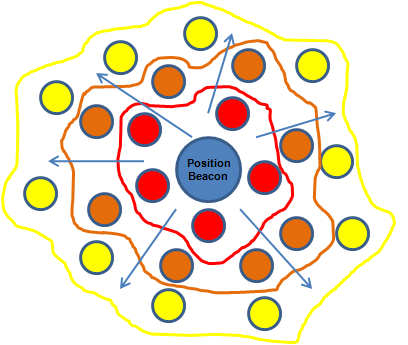
\includegraphics[scale = 0.65]{position_beacon}
\end{figure}
	
	As illustrated on the Figure-xx, suppose that the red agents which are closest ones to the position beacon in the swarm are the only ones which have the capability of interacting with the position beacon. Since the only source of true position measurement is the position beacon, this data must be distributed to these red agents first, then trilateration process must be propogated through the orange agents and then the yellow agents last, since they can only interact with an upper layer in the swarm due to the line of sight and communication range issues.
	
	It is needed to have an algorithm to organize the order of the local trilateration process and the determines the beacon agents for each member of the swarm. Basically this algorithm will assign each agent a rank which represenets the number of sequence in the localization process, and will determine at least three local neighbors of each agent to get in trilateration. Agents which do no have at least three neighbors are assumend to be lost agents and the handling of these type of agents are illustrated in Section -xx.
	
	\paragraph{Routing Algorithm- Bellman Ford}
	As mentioned in the Objectives section of the thesis work, agents are assumed to have a limited communication range and bandwith and the communication topology in the swarm is implemented with a wireless mesh network. In this type of network, each node have a relay in the network and the data is transferred to the related destination with the help of route tables. This makes it possible to have the capability of transferring low bandwith data through the network with multiple hops.  In this work, we implement this topology with a table driven routing scheme known as DSDV(Destination-Sequenced Distance Vector Routing Protocol) algorithm based on Bellman Ford algorithm. Bellman-Ford is and algorithm that computes the shortest path in a weighted graph and the correctness of the algorithm is proven. It is an algorithm based on relaxation, the correct distance to the vertices in the graph are updated iteratively from the initial estimations until converging to the optimal solution. This algorithm is slower than the Djikstra's algorithm which has similar functionalities but negative edge weights can be implemented in the related graph to report the negative cycles which means there is no cheapest path to the related destination vertex. On the other hand, it is possible to augment this algorithm with DSDV implementation to handle the routing loop problem when there is one or more vertices are no more exists in the network. The probability of the case with the non-existence of some vertices during the algorithm is processed can be very high since the agents in the swarm have low sensor capabilities and small range of communication and they have a great possibility to get lost in the environment. A simple demonstration of the Bellman-Ford algorithm with a simple network is illustrated in the Figure-xx
	
\begin{figure}[H]
	\caption{Costs for Shortest Paths to Each Nodes from Node 'S'}
	\centering
	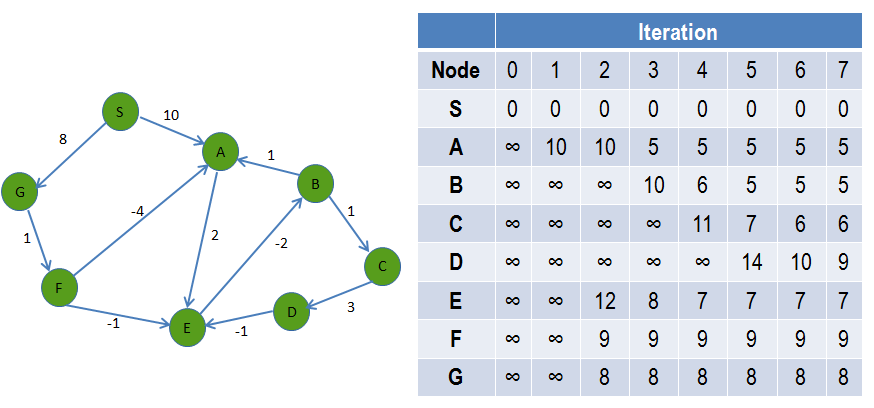
\includegraphics[scale = 0.65]{bellman}
\end{figure}

	
	The algorithm to calculate the shortest paths for node `S` is done at the end of 7 iterations. At the beginning of the process, the weights for each edges are determined including the negative ones and each distance to the paths are filled with infinitive. Then the shortest paths to the each node in the given directed graph are determined iteratively with the help of the Bellman-Ford algorithm 
	
	
	\paragraph{Usage on Bellman Ford algorithm and DSDV}
	
	Bellman Ford algorithm have a drawback related with the routing loop problem which occurs in an event of one or more nodes in the graph are lost during the process. Figure -xx illustrates a simple routing loop problem. 
	
	\begin{figure}[H]
		\caption{Routing Problem Engaged by a Lost of a Node in Network}
		\centering
		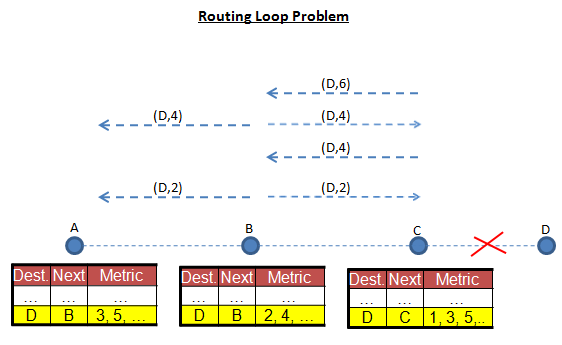
\includegraphics[scale = 0.65]{routing_problem}
	\end{figure}

	

	
	Suppose that the node D have lost its contact with the network due to some malfunction or being lost by getting outside of the communication range to the closest neighbor of itself. Before this event,node C have a unit distance to the node D and consequently node B have a 2 unit distance to node D , node A have a 3 unit distance to node D. In case of a failure on node D, on the next iteration C will update its route table with the 3 unit distance to node D by taking reference the node B. Then node B will update its route table with the shortest distance of 4 units to the node D\ by referencing the node C and this process will diverge to infinity on the shortest paths with the increasing number of iterations. To provide a solution for this type of problems, DSDV algorihm has implement the sequence numbers and counts for hops into the route tables of the nodes. A simple route table for a vertex in a network is given in Figure -xx
		\begin{figure}[H]
			\caption{An Example for Route Table}
			\centering
			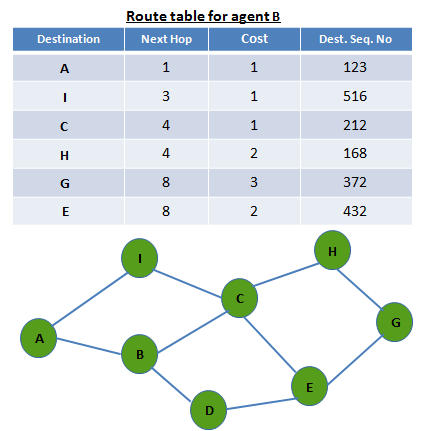
\includegraphics[scale = 0.65]{dest_seq}
		\end{figure}




	
	In the DSDV algorithm, each node have a sequence number and counts for hops (metric) for each route in its route table and periodically transmits the updates including its own sequence number and routing tables updates. In the network, when two routes to the same destination received from two different neighbors the nodes will observe the following rules;
	
	- Choose the one with the larger destination sequence number
	- If the sequence numbers are equal, then choose the route with minimum number of hops and update the route table.
	
		\paragraph{DSDV Link addition}\hspace{0pt} \\
			\begin{figure}[H]
				\caption{An Example for Route Table}
				\centering
				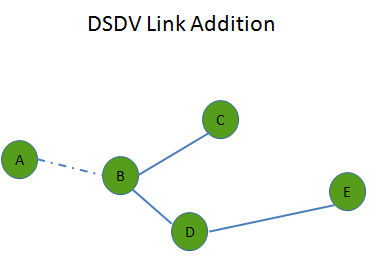
\includegraphics[scale = 0.65]{link_add}
			\end{figure}
	
	When a new node A joins the network, it transmits of its own route table including the destination to itself $<A,A,0,101>$. Then the following procedure will be handled during iterations
	-Node B receives the the transmission of A and inserts a new line into its route table with $<A,A,1,101>$ and propogates this new node to its neighbors
	-Node C and Node D receives this transmission and inserts the new route to their route tables with $<A,B,2,101>$
	
	
	\paragraph{DSDV link breaks}\hspace{0pt} \\
	
			\begin{figure}[H]
				\caption{An Example for Route Table}
				\centering
				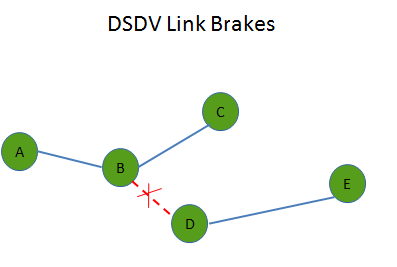
\includegraphics[scale = 0.65]{link_break}
			\end{figure}

	
	When the link between B and D breaks, node B gets no trasnmission from the D and notices the link breaks, then the following procedure will be handled,
	- Node B update the hop count for node D and E to the infinity and increments the sequence numbers to these routes 
	- Node B propogates the updates to its neighbors and node A and node C updates the lines of the routes to the D and E, since the message from B includes higher sequence numbers for those routes. 
	
	DSDV is implementing an algorithm to find the shortest paths between the internal nodes of a given directed graph. The costs for each shortest paths are calculated with the help of the weight of edges in the graph. Since our aim is to find the closest position beacon which has the minimum number of hops, the weight for each edge in the graph must be represented with the same unit size and the directions of the edges are negligible. 
	\subsubsection{Clusters}
	Since there are limited number of position beacons in a swarm, it will be appropriate to cluster the agents around these position agents to minimize the problem to the subproblems in which every one of them there are only one position beacon and the agents which are assigned to that cluster. The error on the trilateration process is expected to be increasing at the lower layers of the process illustrated in Figure -xx because of the cumulative effects of errors added to the position and velocity data of the agents in each layer. Thus, the policy for the assignment of the agents to the clusters must be the number of hops to the routes of position beacons rather than the physical distances. Since DSDV algorithm has a structure storing the number of counts to each route in the tables, this information can be used to determine each agents' clusters in the swarm. 
		\begin{figure}[H]
			\caption{Clusters Around Position Beacons}
			\centering
			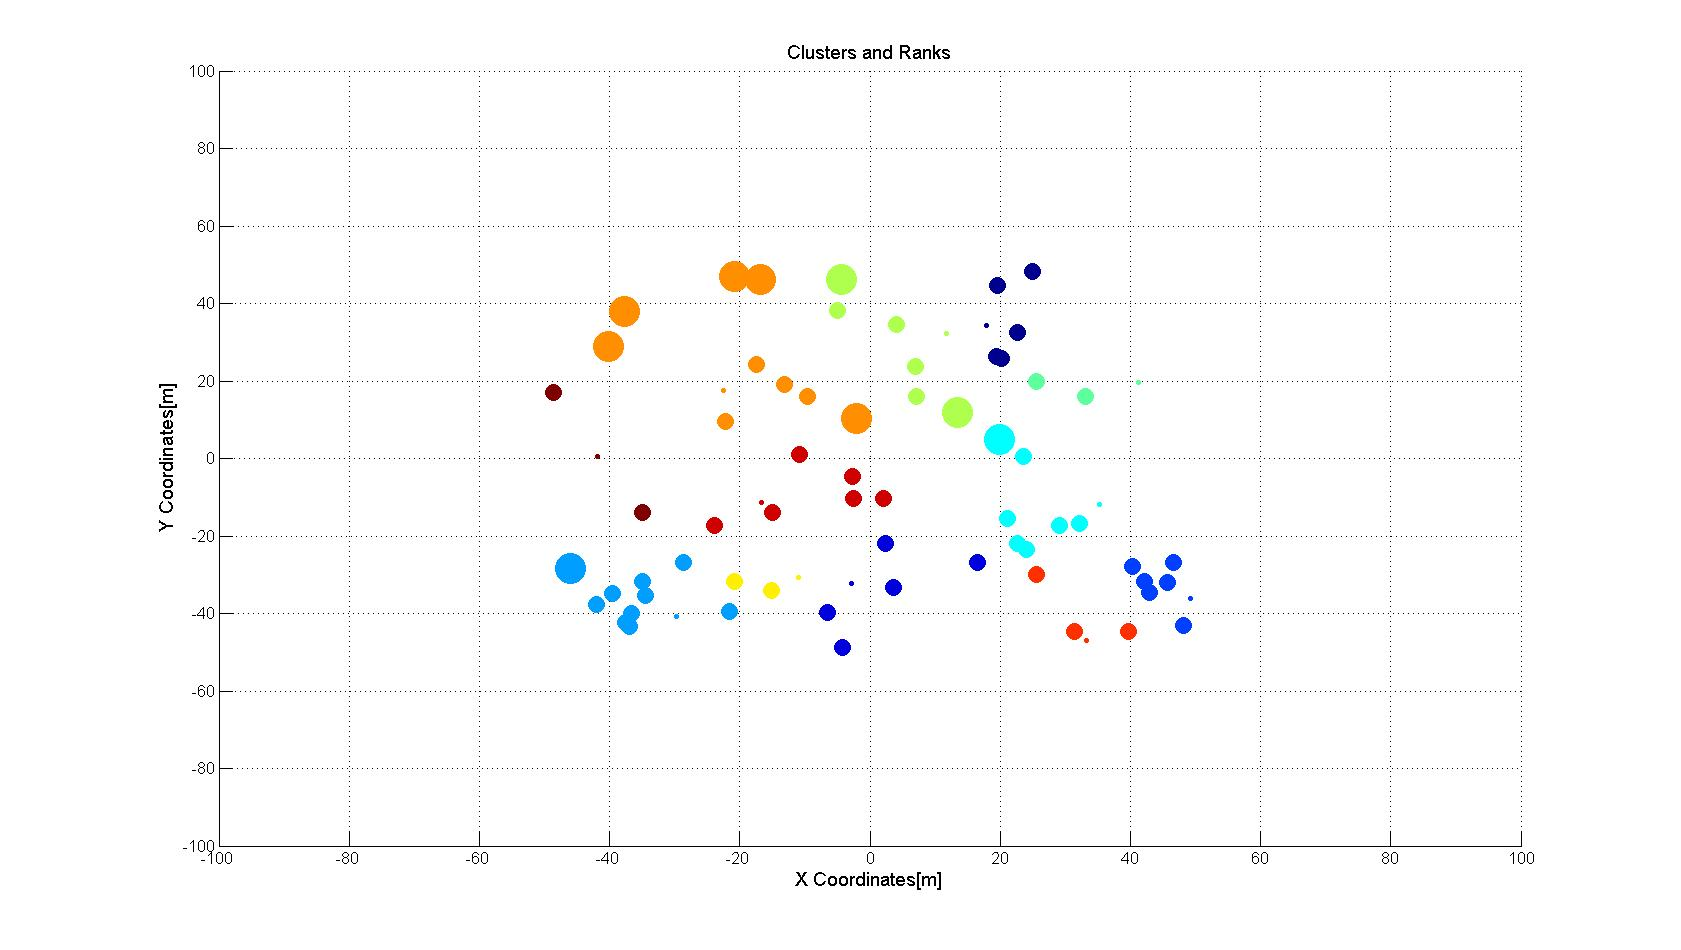
\includegraphics[scale = 0.35]{Clusters_Ranks_2}
		\end{figure}


	
	As illustrated in the Figure -xx, all agents have assigned themselves to the clusters around position beacons, in which they have minimum number of hops in the route to the related position agent.  With this approach, the generic algorithm which will be executed with the period of localization process for each agent must be implemented as follows:
	
	1) Update route table including the routes to the position agents in the swarm with DSDV algorithm 
	2) Check for the routes to the position agents and join the cluster in which minimum number of hops required to that destination.
	3) Wait for the localization sequence in which the agents are entered the process with the increasing number of hops, e.g. the agent which have a single hop to the position agents are processed first, and then the other ones are processed consecutively as illustrated in Figure -xx
	4) If the localization sequence is valid(siranin gelmesi denmeli) for this agent, enter the trilateration process with the agents from upper layer,  which are the next hops in the route table.
	5) Call the update procedure of the observer system of which details are presented in section -xx
	
	\subsubsection{Handling Lost Agents}
	
	The minimum number of neighbors required for the trilateration process is three for a two dimensional localization problem as illustrated in section -xx(trilateration bolumu) . Since the agents are assumed to have a narrow communication range, it is possible to not to find three neighbors for any agent at an instant time. At this case, it will be impossible to relocate these agents with trilateration and the position$\&$velocity data will drift from the real values with the increasing time passed without trilaterions. To avoid these kind of problems, the concept of `lost` agents and the procedures for these type of agents are described as follows:
	
	* An agent gets into 'Lost' mode, if it doesn't find three neighbors at an instant time
	* If an agent is in 'Lost' mode and missed the localization process for three times, it will get into 'Return to Home' mode
	* If an agent is in 'Return to Home' mode, it will directly try to reach to the center of the desired formation shape.
	
	The idea behind the 'Return to Home' mode is basically to increase the possibility of the lost agent to get in touch with the rest of the swarm with directing it to the center of the swarm. A simple demonstration of this procedure is illustrated in Figure-xx
	
	
			\begin{figure}[H]
				\caption{Return to Home Approach of a Lost Agent}
				\centering
				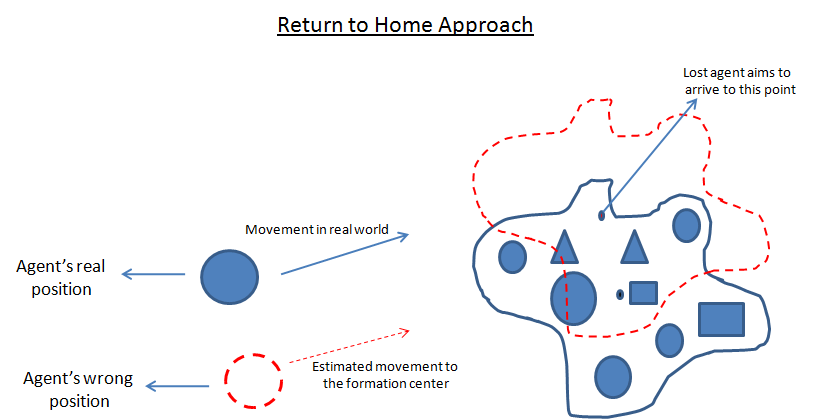
\includegraphics[scale = 0.60]{return_home}
			\end{figure}

	
	
	The lost agent aims to reach to the center of the formation and due to the errors on its position$\&$velocity data, it is expected to arrive to the red point illustrated in the figure. With this maneuver, the lost agent still have a chance to meet some other agents in the swarm even if it directs itself to an incorrect goal state. 
	
	
	\subsubsection{State Estimation Procedure}
	In local positioning subsystem, agents are expected to execute a state estimator algorithm in which they propogate their state vector composed of translational position and velocities with the help of inertial measurements. As discussed in Section 3.1 they will update and correct their positions with the measurements provided by the trilateration process execeuted with the localization timer period of 5 seconds. A Kalman estimator algorithm which uses the trilateration outputs as external measurents and the sensor measurement as inputs is designed to fusion the sensor measurements with the trilateration calculations. The model for this observer system is defined as follows:
	
	The state vector for each agent is defined as:
	\begin{equation}
        x_k = \begin{bmatrix}
            X_k \\
            \dot{X}_k\\
                \end{bmatrix}
	\end{equation}
	
	where $X_k$ is the position and $\dot{X}_k$ is the velocity of the agents in x coordinates in two dimensional environment. All of the following procedures will be handled exactly the same for the state vector in y coordinates.
	The linear model to propogate states will be:
	\begin{equation}
  x_{k+1} = F_k     x_{k} + B_ku_k + w_k
	\end{equation}
	where $w_k$ is the process noise and 
	\begin{equation}
   F = \begin{bmatrix}
1 & d_t\\
0 & 1
\end{bmatrix}   
	\end{equation}
	
	\begin{equation}
B = \begin{bmatrix}
\frac{{d_t}^2}{2} \\
d_t
\end{bmatrix}
	\end{equation}
	
	\
	where $d_t$ is the propogation period and $u_k$ is the translational acceleration measured by inertial sensors in the x coordinate of the system. The observation which will be calculated with the trilateration process :
	\begin{equation}
z_k = H_kx_k + v_k
	\end{equation}
	where $v_k$ is the measurement noise and since the trilateration process will provide new position informations of the agents:
	\begin{equation}
H_k = \begin{bmatrix}
1\\0
\end{bmatrix}
	\end{equation}
	The noise models for the process and the measurement are modelled with:
	\begin{equation}
 w_k = \mathcal{N}(\mathbf{0,Q_k})
	\end{equation}
		\begin{equation}
		v_k = \mathcal{N}(\mathbf{0,R_k})
		\end{equation}
		where $w_k$ is the process noise with zero mean multivariate normal distribution with covariance of $Q_k$ and $v_k$ is the measurement noise with zero mean Gaussian distribution with a covariance of $R_k$
		
		The filter has two main subsections named predict and update phases. The update phase of the filter is executed after each trilateration process with a period of 5 seconds. The filter equations are as follows:
		
		Propogation phase:
		\begin{equation}
    \hat{x}_{k,k-1} = F_k\hat{x}_{k-1,k-1} + B_ku_k
		\end{equation}
		\begin{equation}
 P_{k,k-1} = F_k P_{k-1,k-1}F^T_k + Q_k
		\end{equation}
		
		Update Phase:
		\begin{equation}
\tilde{y}_k = z_k - H_k  \hat{x}_{k,k-1} 
\end{equation}
	\begin{equation}
S_k = H_k P_{k,k-1} H^T_k + R_k
\end{equation}
	\begin{equation}
K_k =  P_{k,k-1} H^T_kS_k^{-1}
		\end{equation}
		\begin{equation}
 \hat{x}_{k,k} =  \hat{x}_{k,k-1} + K_k \tilde{y}_k
		\end{equation}
		\begin{equation}
P_{k,k} = (I - K_kH_k)P_{k,k-1}
		\end{equation}
		
		
		where $Q_k$ is the process covariance matrix and $R_k$ is the measurement covariance chosen as 
		\begin{equation}
Q_k = \begin{bmatrix}
Max. Acceleration Error * \frac{d^2_t}{2} & 0 \\
0 & Max. Acceleration Error * d_t
\end{bmatrix}
		\end{equation}
		\begin{equation}
R_k = Max. Position Error on Trilateration Process
		\end{equation}
		
	in the above equations $K_k$ represents the Kalman gain matrix and $S_k$ is the residual covariance of the system at time $k$. $\hat{x}_{k,k}$ is the posteriori state estimate updated with measurements at time $k$ ;  $\hat{x}_{k,k-1}$ is the priori estimate of the state vector predicted with inputs at time $k$; $P_{k,k}$ is the posteriori error covariance matrix updated with measurements at time $k$; $P_{k,k-1}$ is the priori estimate covariance predicted with the inputs at time $k$
		
		
\subsection{FORMATION CONTROL}		
  The details of the methodology for dynamical formation control with heterogenous mobile robots is presented in this chapter. Basically three different approaches as artificial forces method, bubble packing method and randomized fractals method are implemented. It is possible to classify these methods in two sub categories. Potential field based approaches implements artificial forces acting on agents to get inside and cover the desired formation shape homogenously by avoiding collisions between the agents. The resultant positions of the agents in the formation shape is not certain, it dynamically changes with the instantaneous positions and interactions of the agents with each other and environment. The other two methods , shape partitioning based approaches, share a common structural basis. In these approaches the complex formation shape is partitioned into goal states to cover the shape homogenously with the mobile robots. The assignment of the agents to these goal states is handled with special algorithms to optimize the overall energy consumpytion of the swarm. The difference between these two methods is the partitioning approach of the complex shape. 
		
	\begin{figure}[H]
		\caption{Clusters Around Position Beacons}
		\centering
		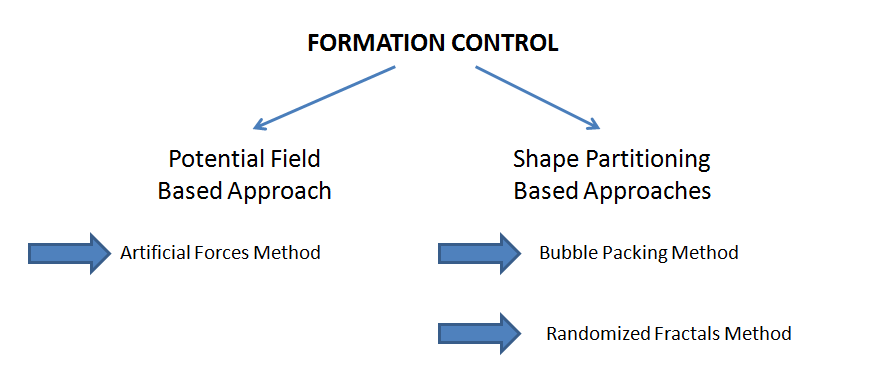
\includegraphics[scale = 0.60]{methods}
	\end{figure}

		
		
		\subsubsection{Potential Field Based Approach}
		\paragraph{Artificial Forces Method}
		Artificial forces method implements some potential fields over each agent arised from the interactions between agents, formation shape and environment etc. The positions of the agents at the formation shape  are determined randomly with a local equilibrium point of the swarm in which every agent is at balance under the total force acting from the environment. There are basically three different kinds of artificial forces named intermember forces representing the forces created by the other agents in the swarm to achieve collision avoidance, the attractive forces representing the forces created by the desired formation shape to attract the agent into the shape and repulsive forces created by the formation shape to keep agent inside the shape. It is possible to augment these type of forces for specific tasks and objectives, e.g. obstacle forces created by the obstacles in the environment can be implemented to achieve obstacle avoidance.
		Since the method to calculate the artificial forces involves contour integrals, it will be useful to give mathematical definition of contour integrals;
		
		Consider a curve $C$ which is a set of points $z = (x,y)$ in the complex plane defined by
		\begin{equation}
x = x(t),   \hspace{0.1cm} y = y(t),  \hspace{0.1cm} a\leq t \leq b
		\end{equation}
		where $x(t)$ and $y(t)$ are continuous functions of the real parametere t.  It is possible to write
		
		\begin{equation}
z(t) = x(t)+iy(t),   \hspace{0.1cm} a\leq t \leq b
		\end{equation}
		
		This curve is called smooth if $z(t)$ has continuous derivative $z'(t) \neq 0$ for all points along the curve, and it is called simple if it does not cross itself as mentioned;
		\begin{equation}
z(t_1) \neq z(t_2)   \hspace{0.1cm} whenever   \hspace{0.3cm} t_1\neq t_2
		\end{equation}
		On the other hand if  $z(a)=z(b)$ is the only intersection point, the curve is said to be simple closed curve. Regarding with these given definitions, an example for a  simple smooth closed curve is illustrated in Figure -xx
			\begin{figure}[H]
				\caption{A Simple Closed Curve}
				\centering
				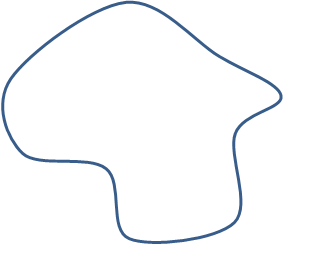
\includegraphics[scale = 0.60]{simple_closed_curve}
			\end{figure}

		
		
		Let $f(z)$ is a complex function in a domain $D$ in the complex pane and let $C$ be simple closed contour contained in $D$ with initial point $z_0$ and terminal point  $z$. It is possible to take the integral of $f(z)$ along the contour $C$
		
		\begin{equation}
    \oint_C f(z) dz = \int_{a}^{b} f(z(t))\frac{dz(t)}{dt} dt
		\end{equation}
		where
		\begin{equation}
\frac{dz(t)}{dt} = \frac{dx(t)}{dt} + i\frac{dy(t)}{dt},   \hspace{0.1cm} a\leq t\leq b
		\end{equation}
		
		To simplify this equation, one can wrtie $f(z) = u(x,y) + iv(x,y)$ and $dz = dx + idy$ into the statements,
		
		\begin{align*}
\oint_C f(z)dz & = \oint_C u dx - v dy + i \oint_C u dy + v dx \\
                        &= \int_{a}^{b}\left[u(x(t),y(t) )\frac{dx(t)}{dt} - v(x(t),y(t) )\frac{dy(t)}{dt}\right]dt\\
                        & \hspace{0.4cm} + i\int_{a}^{b} \left[u(x(t),y(t) )\frac{dy(t)}{dt} + v(x(t),y(t) )\frac{dx(t)}{dt}\right]dt
		\end{align*}
		
     \subparagraph{Utitilty Functions}\hspace{0pt} \\
		As it is mentioned in the Section-xx Objectives part, the formation shapes will be complex contours which cannot be identified analytically, but the definition for the artificial forces and utility functions are expressed in continuous contour integrals which requires the analytical expression of the curve on which the integral will be taken. To enable these type of calculations it is required to provide these statements in discrete domain to achieve calculations with complex closed curves. \\ \newline
\textit{ 		1- Cauchy Winding Number:} \\ 
		Cauchy winding number of a curve in the plane around a given point is the number of times that curve travels counterclockwise around the point. This number is used to switch on/off some of the artificial forces while the agent is inside or outside of the formation shape. Suppose $C$ is the complex closed curve which is a set of points $z=(x,y)$ in the complex plane  and $z_i$ is a point to check whether it is inside of the curve, then the Caucy winding number is :
					
		\begin{equation}
 n(C,z_i) = \frac{1}{2\pi i}\oint_C \frac{dz}{z-z_i}
 		\end{equation}
		
		The winding number for agent $i$ in the swarm,
\begin{equation}
n(C,z_i) = \left\{ \begin{array}{rl}
1 &\mbox{ when member i is inside C} \\
0 &\mbox{ when member i is outside C}
\end{array} \right.
\end{equation}
		To implement this statement in discrete domain 
		\begin{equation}
n(C,z_i) = \frac{1}{2\pi i} \oint_C f(z)dz
		\end{equation}
		where 
		\begin{equation}
f(z) = \frac{1}{z-z_i}
		\end{equation}
		Function of $f(z)$ can be partitioned into real and complex parts as:
		\begin{equation}
u(x,y) = real(f(z))  \hspace{0.2cm} and \hspace{0.2cm} v(x,y) = imag(f(z))
		\end{equation}
		
		partitioning as it mentioned in equation -xx
		\begin{equation}
\oint_C f(z)dz  = \oint_C u dx - v dy + i \oint_C u dy + v dx 
		\end{equation}
		then
		\begin{equation}
n(C,z_i)  = \frac{1}{2\pi i} \left[\int_{a}^{b} \left(u\frac{dx}{dt} - v\frac{dy}{dt}\right)dt + i\int_{a}^{b}\left(u\frac{dy}{dt} + v\frac{dx}{dt}\right)dt\right]
		\end{equation}
		
		This contour integral representation of this equation is
		
		\begin{equation}
n(C,z_i)  = \frac{1}{2\pi i} \left[\sum_{k=1}^{K} \left(u(x_{k+1} - x_k ) - v(y_{k+1} -yx_k )\right) + i\sum_{k=1}^{K}\left(u(y_{k+1} - y_k ) + v(x_{k+1} - x_k )\right)dt\right]
		\end{equation}
		where
		\begin{equation}
z_k - z_{k-1} = z_{k+1} - z_k, \hspace{0.2cm}  \forall k ;  \hspace{0.2cm} when  \hspace{0.2cm} K \to\infty
		\end{equation}

		
The assumption of $K \to\infty$ makes it possible to calculate the integral of Cauchy winding number with a small error with large number of $K$ which can be achieved by partitioning the desired formation shape  into small pieces with equal  distances. This approach is used to provide representations of the contour integrals in discrete domain. 

			\begin{figure}[H]
				\caption{Formation Shape in an Environment (Green Dots: Inside of the Shape - Red Dots: Outside of the Shape)}
				\centering			
				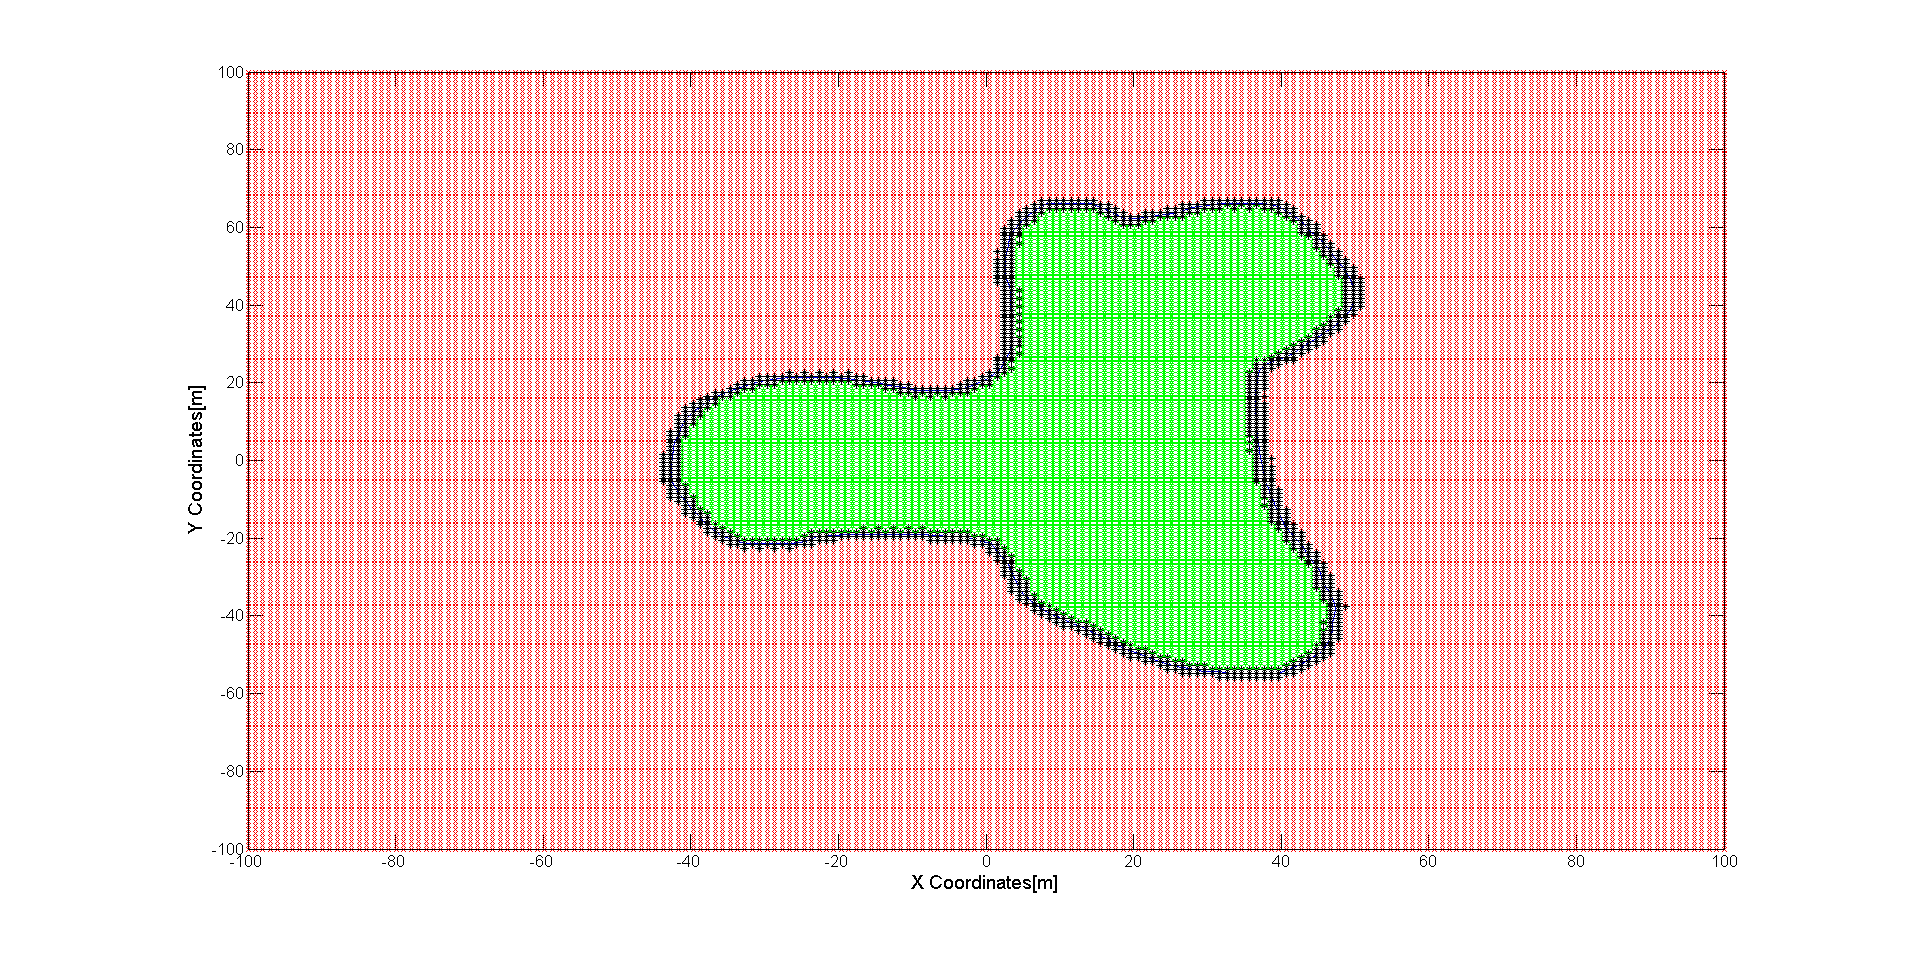
\includegraphics[scale = 0.30]{iceride_disarida}

			\end{figure}


		\textit{ 	2- Length of a formation shape} \\ 
		
		
		The length of a formation shape can be calculated with the equation of;
		
		\begin{equation}
       l(C)= \oint_C \norm{dz}
		\end{equation}
		
		the expression for this contour integral with points of   $z_k = (x_k,y_k)$ in the complex plane
		\begin{equation}
l(C) = \sum_{k=1}^{K}\sqrt{(x_{k+1} - x_k)^2 + (y_{k+1} - y_k)^2}
		\end{equation}
				where
				\begin{equation}
				z_k - z_{k-1} = z_{k+1} - z_k, \hspace{0.2cm}  \forall k ;  \hspace{0.2cm} when  \hspace{0.2cm} K \to\infty
				\end{equation}
		
	
		\textit{ 	3-Center of a Formation Shape} \\ 	
	The center of a formation shape can be calculated with the equation of;
	\begin{equation}
 z_c = \frac{\oint_C z\norm{dz}}{l(C)}
	\end{equation}
		
				the expressiion for this equationl with points of  $z_k = (x_k,y_k)$ in the complex plane
				\begin{align*}
&z_{cx} = \frac{\sum_{k=1}^{K}x(k)}{K}  \\
&z_{cy} = \frac{\sum_{k=1}^{K}y(k)}{K}  
				\end{align*}
		
		where $z_{cx}$ and $z_{cy}$ are the $x$ and $y$ coordinates of the center of formation shape respectively.
		
	
		\textit{ 	4- Area of a Formation Shape} \\ 		
		Green's theorem can be used to calculate of the area of a closed curve. According to this theorem the area of $D$ given by the double integral
		\begin{equation}
 A = \int\int_D dA
		\end{equation}
		can be calculated with the line integral of
		\begin{equation}
 A = \oint_D F ds = \frac{1}{2} \oint_D xdy - ydx
		\end{equation}
where
\begin{equation}
F(x,y) = (-y/2,x/2)
\end{equation}
		
	This contour integral can be reduced down to
	\begin{align*}
Area &= \frac{1}{2} \oint_C xdy - \frac{1}{2} \oint_C ydx \\
&= \frac{1}{2} \int_{t=a}^{b} x(t)\frac{dy(t)}{dt}dt - \frac{1}{2} \int_{t=a}^{b}y(t)\frac{dx(t)}{dt}dt
	\end{align*}
		
			the expressiion for this equationl with points of  $z_k = (x_k,y_k)$ in the complex plane
			
			\begin{equation}
       Area = \frac{1}{2} \sum_{k=1}^{K} x_k(y_{k+1} - y_k) - \frac{1}{2} \sum_{k=1}^{K}y_k(x_{k+1} - x_k)
			\end{equation}
			
				where
				\begin{equation}
				z_k - z_{k-1} = z_{k+1} - z_k, \hspace{0.2cm}  \forall k ;  \hspace{0.2cm} when  \hspace{0.2cm} K \to\infty
				\end{equation}
 \subparagraph{Artificial Forces}\hspace{0pt} \\

			Artificial forces are defined to gather the agents in the swarm inside a formation shape and make them distributed homogenously inside the shape. It is possible to define some additional artificial forces to implement features like obstacle$\&$collision avoidance or smooth transitions between the boundaries of the formation shape. Attractive forces, repulsive forces, intermember forces, obstacle forces and transition forces are implemented to generate individual control laws for all agents in the swarm. Suppose the state of a member $i$ is described by
			\begin{equation}
X_i = \begin{bmatrix}
z_i\\ \dot{z}_i
\end{bmatrix}
			\end{equation}
			where  $z_i \in C$, represents the position of the $i^{th}$ member of the swarm and $\alpha = \begin{bmatrix}
1 & 0
			\end{bmatrix}$ and $\beta = \begin{bmatrix}
0 & 1
			\end{bmatrix}$. The state of the whole swarm $x= \begin{bmatrix}
X_1 & X_2 & ... X_n
			\end{bmatrix}$ is determined by the linear equations of [pubudu referans verelim]
			\begin{equation}
\dot{x} = Ax + Bu
			\end{equation}
			where
			\begin{align*}
&A = diag\left(\hat{A}\right)_{nxn}\\
&B = \frac{1}{m} diag\left(\hat{B}\right)_{nxn}
			\end{align*}
			with
			\begin{equation}
\hat{A} = \begin{bmatrix}
0&1\\0&0
\end{bmatrix} , \hspace{0.2cm} \hat{B} = \begin{bmatrix}
0&1
\end{bmatrix}
			\end{equation}
			
			The vector for individual control laws of the swarm
			\begin{equation}
u = \begin{bmatrix}
u_1 & u_2 & ... & u_n
\end{bmatrix}
			\end{equation}
			where
			\begin{equation}
u_i = F_{i,a} + F_{i,r} + F_{i,m} + F_{i,t}
			\end{equation}
		It is necessary to define the concept of "covearge circle"	for the agents which will be used in the artificial forces calculations. Coverage circle of agent $i$, $C_i$ is defined as the circle with minimum radius which can cover the whole agent's collision surface. The radius of this circle is given with $d_c$. Some of the examples of coverage circles for different types of mobile robots are illustrated in Figure -xx below
		
					\begin{figure}[H]
						\caption{Coverage Circles of Different Types of Agents}
						\centering
						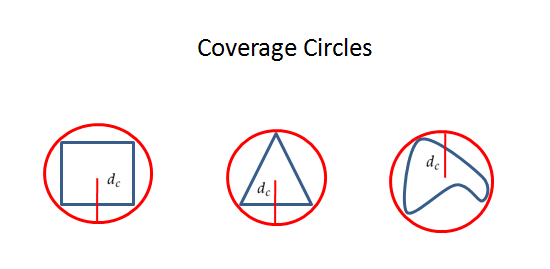
\includegraphics[scale = 0.60]{coverage_circles}
					\end{figure}
		

		
		
		The components of these  control forces are described in details at the following section. \newline
				\textit{			1- Attractive Forces} \\ 

			Attractive forces are the artificial force components generated by the formation shape to attract the agent towards the center of the formation .They are active when the agents are outside of the shape. 
						\begin{figure}[H]
							\caption{Attractive Forces Generated by the Formation Shape}
							\centering
							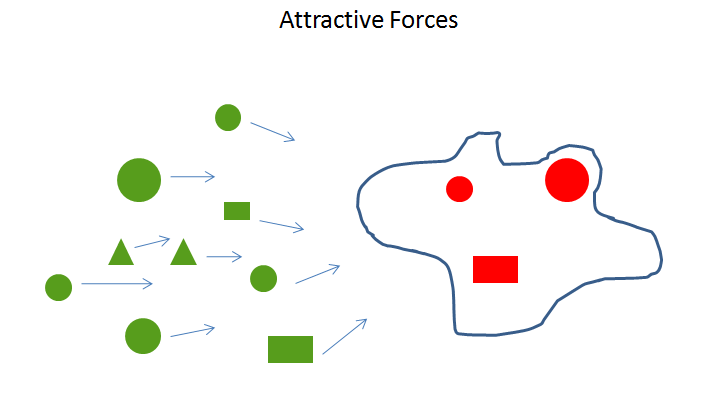
\includegraphics[scale = 0.60]{attractive_forces}
						\end{figure}	



The equations for the attractive forces are defined as follows:			
			\begin{equation}
F_{i,a} := \frac{k_a (1-n(C,\alpha X_i))}{l(C)} \oint_C(z-\alpha X_i)\norm{dz}
			\end{equation}
			where $k_a$ is the variable gain for the attractive forces. The representation of the attractive forces on agent $i$ on $z_i = (x_i, y_i)$ with the points of  $z_k = (x_k,y_k)$ of formation shape in the complex plane:
			\begin{align*}
& F_{iax} =\frac{k_a (1-n(C,\alpha X_i))}{l(C)}  \sum_{k=1}^{K} (x_k  - x_i)\\
& F_{iay} =\frac{k_a (1-n(C,\alpha X_i))}{l(C)}  \sum_{k=1}^{K} (y_k  - y_i)\\
			\end{align*}
			where
		\begin{equation}
		z_k - z_{k-1} = z_{k+1} - z_k, \hspace{0.2cm}  \forall k ;  \hspace{0.2cm} when  \hspace{0.2cm} K \to\infty
		\end{equation}
			
			and $F_{iax} , F_{iay} $ are the attractive force components in $x,y$ coordinates respectively.\newline
			
					\textit{	2- Repulsive Forces} \\ 
		
			Repulsive forces are the artificial force components generated by the formation shape to keep the agents inside the shape. They are active when the agents are inside the shape. 
					
							\begin{figure}[H]
								\caption{Repulsive Forces Generated by the Formation Shape}
								\centering
								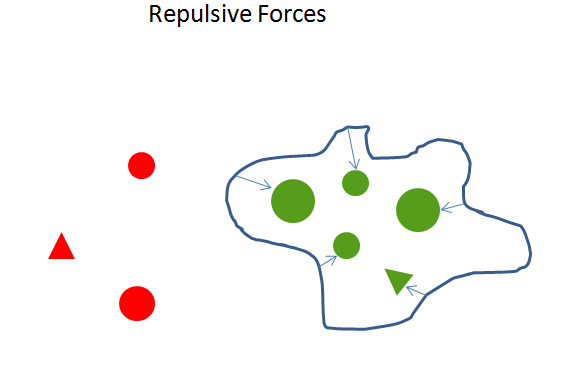
\includegraphics[scale = 0.60]{repulsive_forces}
							\end{figure}
							
			The equations for the attractive forces are defined as follows:	
				\begin{equation}
F_{i,r} := k_r  n(C,\alpha X_i) \oint_C \left[\frac{\alpha X_i - z}{\norm{\alpha X_i - z}^3}\right] \norm{dz}
				\end{equation}
			where $k_r$ is the variable gain for the repulsive forces. The representation of the repulsive forces on agent $i$ on $z_i = (x_i, y_i)$ with the points of  $z_k = (x_k,y_k)$ of formation shape in the complex plane:
				\begin{align*}
				& F_{irx} = k_r n(C,\alpha X_i)  \sum_{k=1}^{K} \frac{x_i - x_k}{\norm{\alpha X_i - z_k}^3}\\
				& F_{iry} = k_r n(C,\alpha X_i)  \sum_{k=1}^{K} \frac{y_i - y_k}{\norm{\alpha X_i - z_k}^3}
				\end{align*}
						where
						\begin{equation}
						z_k - z_{k-1} = z_{k+1} - z_k, \hspace{0.2cm}  \forall k ;  \hspace{0.2cm} when  \hspace{0.2cm} K \to\infty
						\end{equation}
						
						and $F_{irx} , F_{iry} $ are the repulsive force components in $x,y$ coordinates respectively. \newline
						
					\textit{		3- Inter-member repulsion forces} \\ 
	
			Intermember forces are the artificial force components generated by the agents in the swarm to avoid collisions between themselves. 
			
			\begin{figure}[H]
				\caption{Intermember Forces Generated by Agents}
				\centering
				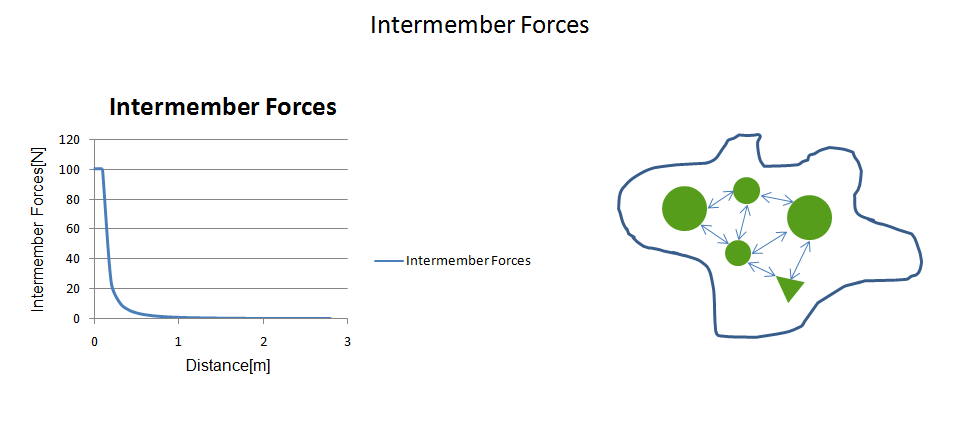
\includegraphics[scale = 0.60]{intermember_forces}
			\end{figure}
			
			The equations for the intermember forces on the agent $i$ on $z_i = (x_i, y_i)$  in the complex plane ,
			
			\begin{equation}
F_{i,m} = k_m \sum_{j=1, j\neq i}^{N}\frac{\alpha X_i - \alpha X_j}{(\norm{\alpha X_i - \alpha X_j})} \frac{1}{(\norm{\alpha X_i - \alpha X_j} - d_o)^2}
			\end{equation}
			where $d_o$ is the total distance minimum distance between the agents which can be calculated with
			\begin{equation}
 d_o = d_i + d_j
			\end{equation}
			The force components in x,y coordinates respectively,
			\begin{align*}
&F_{imx} = k_m \sum_{j=1, j\neq i}^{N}\frac{x_i- x_j}{\norm{\alpha X_i - \alpha X_j}}  \frac{1}{(\norm{\alpha X_i - \alpha X_j} - d_o)^2}\\
&F_{imy} = k_m \sum_{j=1, j\neq i}^{N}\frac{y_i- y_j}{\norm{\alpha X_i - \alpha X_j}}  \frac{1}{(\norm{\alpha X_i - \alpha X_j} - d_o)^2}\\
			\end{align*}
			where $k_m$ is the variable gain for the intermember forces.  \newline
			
					\textit{4- Transition Forces} \\ 
			
			
			Transition forces are the artificial force component to force the agent inside the formation shape when they are close to the boundaries. Since the attractive forces have a decreasing nature while the agent getting closer to the formation shape, it is needed to add this type of forcing function to ensure the agents to get inside the shape. Transition forces are active outside of the desired formation shape.
			
				\begin{figure}[H]
					\caption{Comparison of Attractive and Transition Forces Close to the Formation Shape Boundary}
					\centering
					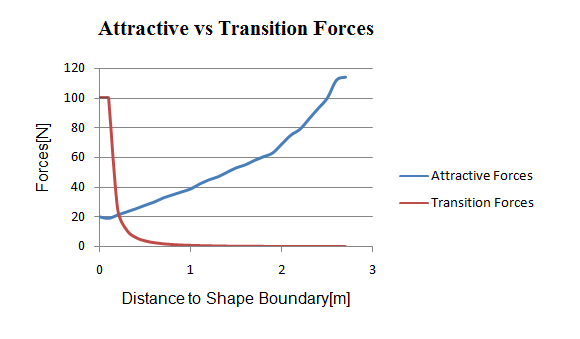
\includegraphics[scale = 0.80]{transition_forces}
				\end{figure}
			
			
				The equation for the transition forces are defined as follows:	
				
				\begin{equation}
 F_{i,t} = k_t (1-n(C,\alpha X_i) \oint_C \frac{z-\alpha X_i}{\norm{z-\alpha X_i}}\norm{dz}
				\end{equation}
				where $k_t$ is the variable gain for the transition forces. The representation of the transition forces on agent $i$ on $z_i = (x_i, y_i)$ with the points of  $z_k = (x_k,y_k)$ of formation shape in the complex plane:
			
\begin{align*}
&F_{itx} = k_t  (1-n(C,\alpha X_i) \sum_{k=1,}^{K}\frac{x_k- x_i}{\norm{\alpha X_i - z_k}^3}\\
&F_{ity} = k_t  (1-n(C,\alpha X_i) \sum_{k=1,}^{K}\frac{y_k- y_i}{\norm{\alpha X_i - z_k}^3}\\
\end{align*}
			
			where  $F_{itx} , F_{ity} $ are the transition force components in $x,y$ coordinates respectively. \newline
			
					\textit{			5- Obstacle forces} \\ 

			
			Obstacle forces are the artificial force components generated by the obstacle in the environment to achieve obstacle avoidance of the agents during formation control. 	
			The equation for the obstacle forces are defined as follows:	
			
			\begin{equation}
F_{i,o} := k_o  \oint_O \left[\frac{\alpha X_i - z_o}{(\norm{\alpha X_i - z_o} - d_{ci})^4}\right] \norm{dz_o}
			\end{equation}
			where $k_o$ is the variable gain for the transition forces and $d_{ci}$ is the radius of coverage circle of agent $i$ . This contour integral is taken on the curve of the obstacle with  points of $z_o = (x_o,y_o)$ in the complex plane.
			
			The representation of the obstacle forces on agent $i$ on $z_i = (x_i, y_i)$ with the points of  $z_{ok} = (x_{ok},y_{ok})$ of formation shape in the complex plane:
			\begin{align*}
			& F_{iox} = k_o   \sum_{k=1}^{K} \frac{x_i -x_{ok}}{(\norm{\alpha X_i - z_{ok}} -d_{ci})^4}\\
			& F_{ioy} = k_o   \sum_{k=1}^{K} \frac{y_i - y_{ok}}{(\norm{\alpha X_i - z_{ok}} -d_{ci})^4}\\
			\end{align*}
			
			where
			\begin{equation}
		z_{ok}- z_{ok -1} = z_{ok+1} - z_{ok}, \hspace{0.2cm}  \forall k ;  \hspace{0.2cm} when  \hspace{0.2cm} K \to\infty
			\end{equation}
			
			
			\subparagraph{Buffer Zone Implementation}\hspace{0pt} \\
			
     The attractive and transition forces are defined to be active when the agents are outside of the shape, the resistive forces are active when agents are inside the shape. Due to this type of sharp transitions on the total artificial force acting on an agent which is crossing the boundary of the formation shape, it is possible to have a chattering effect. To avoid this chattering effect and provide a smooth transition of the agent to pass the boundary of formation shape, a buffer zone around the boundaries are implemented. The main approach during the transition of these boundaries is to dynamically change the variable gains of these artificial forces to linearly change between zero and nominal values at the boundary conditions. 
     
			\begin{figure}[H]
				\caption{Transition of the Artificial Forces on Buffer Zone}
				\centering
				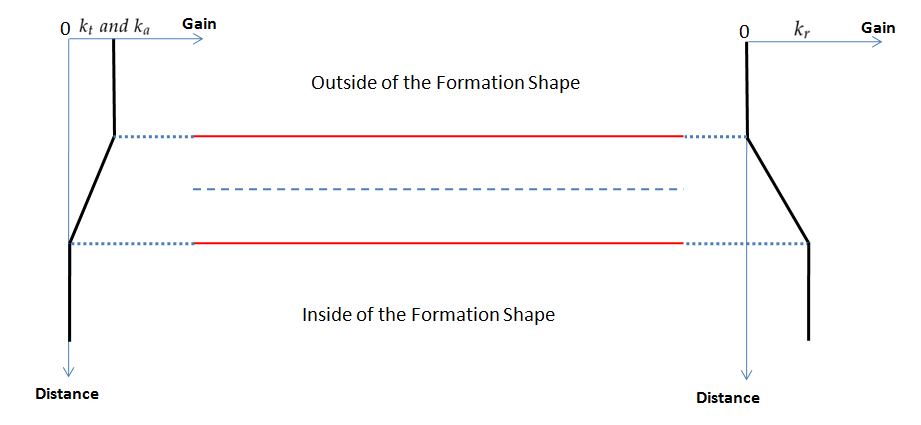
\includegraphics[scale = 0.50]{buffer_zone}
			\end{figure}
			
			
			\subparagraph{XSwarm Theory}\hspace{0pt} \\

			
			Samitha and Pubudu [xx] have provided a definition of "X-Swarm" and give a theorem which describes the motion of an agent towards s the formation shape based on the X -Swarm definition. Let $S$ be a swarm with $N$ agents. This swarm is defined as X-Swarm if there exists some positive constants $\delta$ and  $ \gamma$ that satisfy the following conditions simultaneously for all $i,j \in S$ and $i \neq j$
			
\begin{align*}
&\succ\hspace{0.2cm}  d_{ij} \geq \gamma + \delta \\
&\succ \hspace{0.2cm}   \norm{\frac{z_i - z_{cm}^i}{z_i - z_{cm}}} < \left(1+\frac{\delta}{\gamma}\right)^3
\end{align*}
			where
\begin{equation}
 d_{ij} = \norm{z_i - z_j} and z_{cm}^i = \frac{\sum_{j=1; j\neq i}^{N} z_j}{N-1}
\end{equation}
The term of $z_{cm}^i$ is the center of mass of the swarm without the $i^{th}$ member.

Lemma 1: The magnitude of artificial inter-member force acting on an agent of X-Swarm  is less than
\begin{equation}
 \frac{k_m(N-1)}{\gamma ^3} \norm{z_i - z_{cm}}
\end{equation}
Proof:

\begin{equation}
 F_{i,m} = k_m \sum_{j=1, j\ neq i}^{N} \frac{z_i - z_j}{d_{ij}^3} 
\end{equation}
Using the first condition of the X-Swarm , we have
\begin{equation}
 \norm{F_{i,m}} < \frac{k(N-1)}{(\gamma + \delta)^3} \norm{z_i - z_{cm}^i}
\end{equation}
Then using the condition 2 of the X-swarm definition, the following expression can be derived

\begin{equation}
 \norm{F_{i,m}} < \frac{k(N-1)}{\gamma^3} \norm{z_i - z_{cm}^i}
\end{equation}
		This result provides an upper bound to the magnitude of the inter-member repulsion force in a X-Swarm.  
		
		Theorem: Conside the agent $i$	outside of a desired formation shape in a X-swarm, if $\frac{k_a}{k_m} > \frac{N-1}{\gamma^3  l(C)}$ then the motion of member $i$ is towards to the center of the swarm. 
		Proof: Choosing a Lyapunov function candidate for the agent $i$ as?
		\begin{equation}
      V_i = \frac{1}{2} \dot{v}_i \dot{v}_i^T + \frac{1}{2} v_i v_i^T\left(k_al(C)-\frac{k_m(N-1)}{\gamma^3}\right) 
      		\end{equation}
			It is possible to show that $\dot{V}_i$ is bounded by taking the derivatives,
			
			\begin{equation}
\dot{V}_i \leq -k_f \norm{\dot{v}^2} + \begin{bmatrix}
\norm{k_m \sum_{j=1, j \neq i}^{N} \frac{z_i - z_j}{\norm{z_i - z_j}^3}} \\
- \frac{k_m(N-1)}{\gamma ^3} \norm{v}
\end{bmatrix} \norm{\dot{v}}
			\end{equation}
			Since agent $i$ is considered a member of a X-swarm, from Lemma -1
			\begin{equation}
\norm{ \sum_{j=1, j \neq i}^{N} \frac{z_i - z_j}{\norm{z_i - z_j}^3}} < \frac{N-1}{\gamma^3} \norm{z_i - z_cm}
			\end{equation}
			and hence
			\begin{equation}
\dot{V}_i < -k_f \norm{\dot{v}_i} ^2
			\end{equation}
			which proves the given theorem.  \newline

	\subparagraph{Implementation of X-Swarm Theory}\hspace{0pt} \\		

Two conditions to create a X-Swarm is to find two positive variables which satisfy the following inequalities

		\begin{align*}
		&\succ\hspace{0.2cm}  d_{ij} \geq \gamma + \delta \\
		&\succ \hspace{0.2cm}   \norm{\frac{z_i - z_{cm}^i}{z_i - z_{cm}}} < \left(1+\frac{\delta}{\gamma}\right)^3
		\end{align*}
		
		It is possible to check the X-swarm conditions for a swarm  with the $min(d_{ij})$ and $max \norm{\frac{z_i - z_{cm}^i}{z_i - z_{cm}}} $ . Lets define the variable  of $X_{sw_{min}}$ and $X_{sw_{max}}$ as following:
		\begin{equation}
X_{sw_{max}} := max \norm{\frac{z_i - z_{cm}^i}{z_i - z_{cm}}}  \hspace{0.2cm} X_{sw_{min}} := min(d_{ij})
		\end{equation}
			To satisfy the X-swarm inequalities, it is possible to write 
			\begin{equation}
 X_{sw_{min}} = \gamma + \delta  \hspace{0.2cm} X_{sw_{max}} = (1 + \frac{\delta}{\gamma})^3
			\end{equation}
			by using the above equations it is possible to calculate the variables of $\gamma$ and $\delta$ can be calculated with,
			\begin{equation}
  \gamma = \frac{ X_{sw_{min}}}{\sqrt[3]{ X_{sw_{max}}}}
			\end{equation}
			and
			\begin{equation}
\delta =  X_{sw_{min}} - \frac{ X_{sw_{min}}}{\sqrt[3]{ X_{sw_{max}}}}
			\end{equation}
			if the calculated  $\gamma$ and $\delta$ are both positive, than the X-swarm conditions are satisfied. Otherwise, the main approach is to increase the variable gain of $k_m$ which determines the magnitude of the repulsive forces between agents to increase the minimum distance between the agents in the swarm, $X_{sw_{min}} := min(d_{ij})$
			
			On the other hand, the theorem related with the convergence of member agents of an X-Swarm to the $z_cm$ is satisfied under the condition of $\frac{k_a}{k_m} > \frac{N-1}{\gamma^3  l(C)}$ . Another approach is to increase the $k_a$ gain to make the related inequality be satisfied to force the agents which are outside of the desired shape to the center mass of the formation geometry. 
			
			
			
		\subsubsection{Shape Partitioning Methods}
			
			Shape partitioning methods have basically reduced down the formation control problem into two subproblems. The first part of the solution is to partition the desired formation shape into potential goal states according to the agent types to cover the desired formation shape homogenously. There are two different solutions to the shape partitioning problem are presented in this thesis work, bubble packing method and randomized fractals method. The second part of the solution is the decision process of the agents to select these goal states continuously to minimize the energy consumption of the swarm. During this decision process, the cost of reaching different goal states will be the main criteria for each agent. It is obvious that each agent will try to choose a goal state with minimum cost according to its position and the orientation in the environment. But the cases in which two or more agents are willing to reach the same goal point must be handled to optimize the overall utility of the swarm. 


Shape partitioning methods have an approach to direct the agents to the goal states in which they have assigned instantly to minimize the energy consumption, but it is important to keep the agents together in the swarm while moving on a trajectory towards the formation shape, to reduce the Lost agent events described in Section-xx. For this purpose, attractive forces which directs the agents to the center of the formation shape under X-swarm consideration is added to the agents' control signal as an additive term. 
			
			\paragraph{Determining the Potential Goal States}
			\subparagraph{Bubble Packing Method} \hspace{0pt} \\	
			
			Bubble packing method is widely used in mesh generation problems. It basically depends on covering a curve, surface or a volume with a proper number of bubbles by packing them tightly which mimic a Voronoi diagram, from which a set of well-shaped Delaunay triangles and tetrahedra can be created by connecting the centers of the bubbles[27].  The algorithm places the bubbles with their initial conditions in the surface and apply them interbubble forces which imitates the Van der Waals forces between the moleculer bonds  to distrubute the bubbles homogenously. Here, the main idea is to generate a mesh for a surface with identical bubbles to mimic a regular Voronoi diagram with the vertices represented by the centers of these bubbles. On the other hand, adaptive population control  methods are developed to increase the number of bubbles to fill the gaps in the shape and to remove the excess bubbles which are overlapping with each other and the shape boundaries. 
			 Since the numbers and the the radius of coverage circles which is defined at Section-xx for the agents are predetermined in our formation control problem, the general bubble meshing algorithm have to be adopted to meet the requirements in shape partitioning in formation control.  The basic approach is to represent the agents in the swarm as bubbles with the radius of  their coverage circles and create a mesh by using these bubbles. \newline
			
			\textit{			I - Initial Placements of the Bubbles} \\ 

		  The initial bubble placements are important because it will greatly reduce the convergence time of the partitioning process. In this work, the bubbles are initiated close to the center of the formation shape randomly. The algorithm for initial bubble placements is provided as follows:
		  

			
			
			\begin{algorithm}[H]
				
				\KwData{Set of Bubbles, Desired Formation Shape }
				\KwResult{Initial Placements of the Bubbles }
				Initialize free configuration space $C_{free}$ as the desired formation shape
				
				\For{<Bubbles of $i$>}
				{		
					*Calculate the free configuration space $C_{free}$ for bubble $i$\;
					 *Put the Bubble $i$ to the closest point to  formation center  $z_c$  in the free configuration space $i$ \;
					 *Add the agent $i$ into the desired formation shape as an obstacle \;
				}
				
				
				\caption{INITIALIZE$\_$BUBBLE$\_$POSITIOINS}
			\end{algorithm}
		
		The term free configuration space $C_{free}$ will be analyzed in detail in Section -xx. An execution of the Algorithm-1 is illustrated in Figure -xx below.
		
				\begin{figure}[H]
					\caption{Initialization of the Bubble Packing Algorithm}
					\centering
					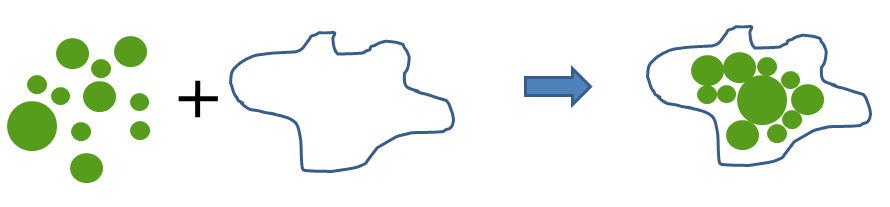
\includegraphics[scale = 0.50]{bubble_packing}
				\end{figure}
				

			\textit{			II- Bubble Meshing Process } \\ 
	
		
		The bubbles are distributed homogenously with this process under two kinds of forces, interbubble forces and shape repulsive forces. The interbubble forces are proximity-based forces so that a system of bubbles is in equilibrium when bubbles are distributed over the whole formation shape. The implemented force equation is given
		
		\begin{equation}
		f_i(l) = \left\{ \begin{array}{rl}
		al^3 + bl^2 + cl + d &\mbox{ when 0 $\leq$ l $\leq$ $l_0$} \\
		0                               &\mbox{ l > $l_0$}
		\end{array} \right.
		\end{equation}
	where $l$ is the distance between the centers of the related bubbles. 
		\begin{figure}[H]
			\caption{Interbubble Forces}
			\centering
			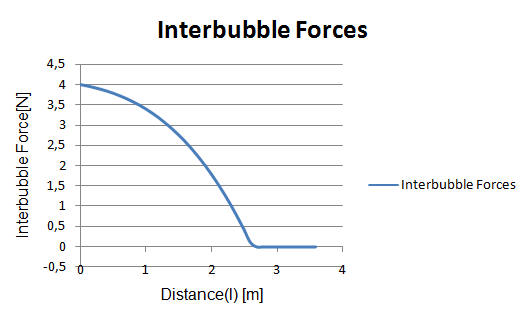
\includegraphics[scale = 0.70]{interbubble_forces}
		\end{figure}
		


	
	The shape repulsive forces have the same characteristics with the repulsive artificial forces discussed in Section -xx. The representation of shape repulsive forces for the desired formation shape $C$ with the points of  $z_k = (x_k,y_k)$ the complex plane::
	
		
			\begin{equation}
			f_r(X_i) := \oint_C \left[\frac{\alpha X_i - z}{\norm{\alpha X_i - z}^3}\right] \norm{dz}
			\end{equation}
			where $k_r$ is the variable gain for the repulsive forces. The representation of the repulsive forces on agent $i$ on $z_i = (x_i, y_i)$ with the points of  $z_k = (x_k,y_k)$ of formation shape in the complex plane:
	
	The bubbles are distributed homogenously under the influence of these two forces when they get an equilibrium state in which the total net forces acting on individual bubbles reaches zero. The final equilibrium states of the bubbles determines the potential goal states of the agents in the swarm to cover the formation shape. 
			\begin{figure}[H]
				\caption{Bubble Packing Algorithm}
				\centering
				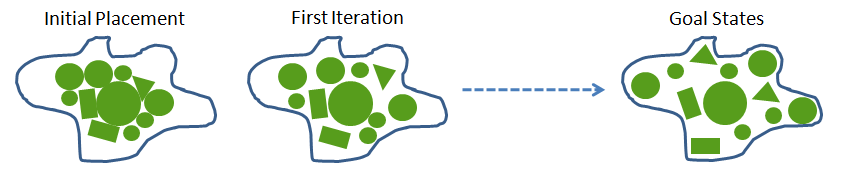
\includegraphics[scale = 0.70]{bubble_packing2}
			\end{figure}


			\subparagraph{Randomized Fractals Method}\hspace{0pt} \\
Randomized fractals method are used to cover surfaces or volumes randomly with fractals. The main idea is to fill the fractals with the areas determined by the rule of [26] :
\begin{equation}
  A_i = \frac{A}{\zeta(c,N)(i+N)^c}
\end{equation}
	where $A$ is the total are to cover and $A_i$ is the area of the $i^th$ fractal. The parameters of $c$ and $N$ can be chosen to implement different changes on the fractals areas with the increasing number of iterations with $c>1$ and $N>0$. Here  $\zeta$ is the Hurwitz function defiend by
	\begin{equation}
  \zeta(c,N) = \sum_{i=0}^{\infty} \frac{1}{(i+N)^c}
	\end{equation}
	It is possble to write, 
	
		\begin{equation}
		\sum_{i=0}^{\infty}A_i = \sum_{i = 0}^{\infty}\left(\frac{A}{\zeta(c,N)(i+N)^c}\right)
		\end{equation}
	
		which tells us the sum of the all areas $A_i$ is the total area of $A$ and the algorithm is space filling. This approach implements the fractals infinitely by reducing the areas in accordance with the Equation -xx to the desired formation shape randomly. 
				\begin{figure}[H]
					\caption{Randomized Fractals}
					\centering
					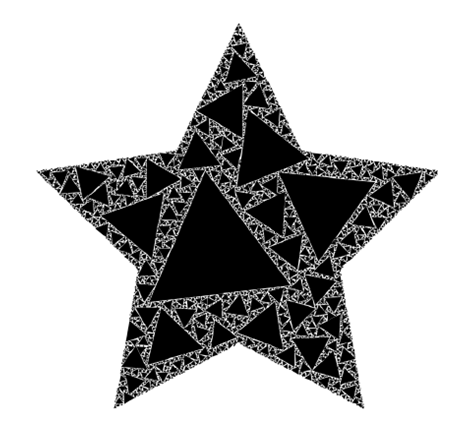
\includegraphics[scale = 0.70]{randomized}
				\end{figure}
		

		
		Since the areas and the number of the agents, which will be represented with their coverage circles, are predetermined in our work, it is possible to adopt this algorithm as follows:
		
					\begin{algorithm}[H]
						
						\KwData{Set of Coverage Circles, Desired Formation Shape }
						\KwResult{Potential Goal States }
						Initialize free configuration space $C_{free}$ as the desired formation shape
						
						\For{<Coverage Circles of $i$>}
						{		
							*Calculate the free configuration space $C_{free}$ for circle $i$\;
						\eIf{$C_{free}  \neq Null$}{
							*Put the circle $i$ randomly in $C_{free}$ \;
								*Add the agent $i$ into the desired formation shape as an obstacle \;
						}{
						  *Break and warn the operator to increase the size of formation shape
						}
												
						}												
						
						\caption{RANDOMIZED$\_$FRACTALS$\_$ALGORITHMS}
					\end{algorithm}
	
	
	\paragraph{Mesh Quality Measurement}\hspace{0pt} \\
	Since we have two different solutions to the shape partitioning problem, it is useful to define a method to compare the performances of these algorithms. One of the criterion of mesh diagrams is topological mesh irregularity [27-29]. This parametere is defined by : 
	\begin{equation}
\epsilon _t = \frac{1}{n} \sum_{i = 0}^{n} |\gamma _i - D|
	\end{equation}
	where 
	
	
			\begin{equation}
			D = \left\{ \begin{array}{rl}
			6                               &\mbox{ for triangles in Voronoi Diagram} \\
			12                             &\mbox{ for tetrahedras in Voronoi Diagram}
			\end{array} \right.
			\end{equation}
	
	and $\gamma _i$ represents the degree, or the number of neighboring nodes connected to the $i^th$ interior node, and $n$ represents the total number of interior nodes, i.e. the number of bubbles or fractals. It is obvious that the topological mesh irregularity vanishes when all nodes have $D$ neighbors, but it is almost not possible in practical application. 
	
		\begin{figure}[H]
			\caption{A Node with 6 Neighbors}
			\centering
			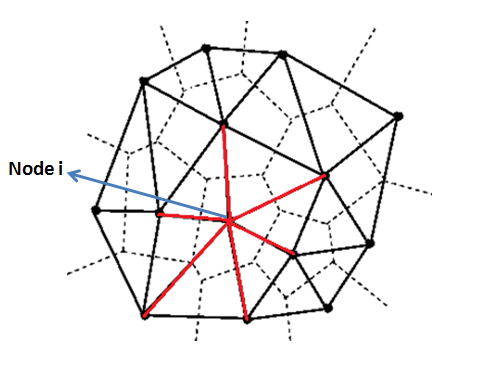
\includegraphics[scale = 0.70]{voronoi}
		\end{figure}

	
	Another metric to evaluate the quality or the performance of the mesh is the geometric irregularity defined as[27]:
	\begin{equation}
\epsilon _g = \frac{1}{m} \sum_{i = 0}^{m} (A-\frac{r_i}{R_i})
	\end{equation}
	where 
		\begin{equation}
		A = \left\{ \begin{array}{rl}
		0.5                               &\mbox{ for triangles in Voronoi Diagram} \\
		\sqrt{2/11}                   &\mbox{ for tetrahedras in Voronoi Diagram}
		\end{array} \right.
		\end{equation}
		
		and $m$ represents the number of nodes, $r_i$ is the radii of inscribed circle of Voronoi cell belonging to node $i$ and $R_i$ is the radii of the circumscribing circle of Voronoi cell belonging to node $i$
	

		\begin{figure}[H]
			\caption{Inscribing and Circumscribing Circle of a Voronoi Cell Belonged to Node i}
			\centering
			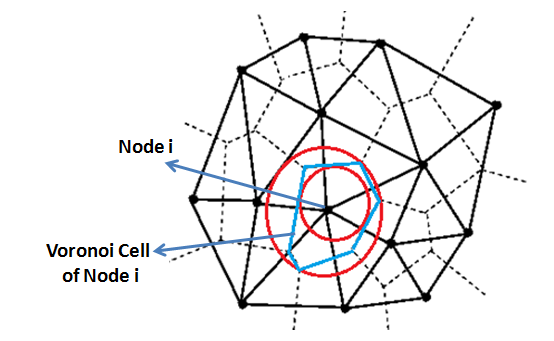
\includegraphics[scale = 0.70]{voronoi2}
		\end{figure}
	
	
		\paragraph{Decision Process on Goal States}\hspace{0pt} \\
	In the first part of the work,Section-xx Shape Partitioning, the formation control problem is reduced down to a problem in which every agent is expected to decide individually where to position in a given set of possible goal states $g_i \in G$ .  During this decision process, the cost of reaching different goal states will be the main criteria for each agent. Given goal states and cost values to these goal states, each agent must individually  decide where to position in the formation. This process must be held to optimize the utility of every agent with a collaboration. It is obvious that some of the agents may want to choose the same goal point to reach, so the swarm must reach a global consensus on target points and conflict cases must be handled. The main approach to provide a solution for this problem is to make each agent to calculate the costs of its own to the goal states and then create a global consensus with the other agents to minimize the overall energy consumption of the swarm while achieving a formation shape. 
	In this work, the cost of reaching a goal state is defined with the minimum shortest path in the environment. A visibility graph based approach is used to calculate the shortest possible path to a goal states by taking into account the obstacles in the environment. The assignment process of the agents to the goal states which will be minimize the overall cost, is handled with the help of Munkres (Hungarian)  algorithm.
	
	\subparagraph{Free Configuration Space}\hspace{0pt} \\
		Since the shortest path is defined in the free configuration domain, each agent must calculate its free space by taking the obstacles in the environment into the account. 

	Assume an environment with set of obstacles $S = \begin{Bmatrix}
	P_1, P_2, .. P_t \end{Bmatrix}$. Configuration for agent $i$ can be described with the position of the center of its coverage circle with $R=\begin{Bmatrix}x_i, y_i\end{Bmatrix}$. Configuration space of $i$ th agent is the environment itself and represented by $C(R_i)$. This configuration space is composed of two subspaces; free configuration space and forbidden configuration space of agent $i$.
	\begin{equation}
	C(R_i) = C_{free}(R_i,S) + C_{forb}(R_i,S)
	\end{equation}
	The configuration space $C(R_i)$ of agent $i$ is the environment itself. If the forbidden space is calculated with Minkowski Sum method, free configuration space can be derived simply by extracting the forbidden space from the environment. Let a single obstacle is described with a point set of $S_1$ and the agent is described with a point set of $S_2$. The Minkowski sum of these two sets $S_1 \subset R^2$ and $S_2 \subset R^2$ can be calculated with the following,
	\begin{equation}
	S_1 \oplus S_2 := \begin{Bmatrix}
	p+q : p \subset S_1, q \subset S_2
	\end{Bmatrix} 
	\end{equation}
	where $p+q$ denotes the vector sum of the vectors $p$ and $q$.
	
	
	\begin{figure}[H]
		\caption{Forbidden Space Caused by an Obstacle}
		\centering
		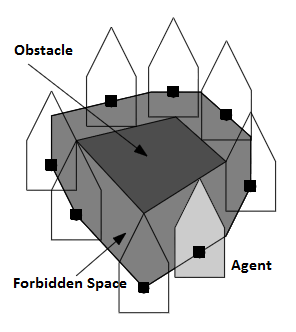
\includegraphics[scale = 0.4]{Forbidden}
	\end{figure}
	Forbidden space for agent $i$, $C_{forb}(R_i, S)$ is the sum of the forbidden spaces calculated for each obstacle in the environment. 
	
		\subparagraph{Visibility Graphs and Dijkstra$'$s Algorihtm}\hspace{0pt} \\
It is obvious that the shortest path between two points in the environment must lie on the free configuration space, $C_{free}$ for each agent. A constraint for the shortest path is given as follows[30] : 
\begin{displayquote}
The shortest path between $p_{start}$ and $p_{goal}$ among a set $S$ of augmented polygonal obstacles consists of the arcs of the visibility graph $\gamma_{vis}(S^*)$ where $S^* := S \cup \begin{Bmatrix}
p_{start}, p_{goal}
\end{Bmatrix}$
\end{displayquote}
A visibility graph,$\gamma_{vis}(S^*)$ , is a graph which is set of interior nodes representing the vertices of the set of obstacles, $S$, in the environment and edges which represents visible (which are not crossing and interior region of an obstacel) connections between these nodes. 

Consider set of obstacles in the environment is augmented with the Minkowski Sums described in the Section-xx . Let these set of augmented polygonal obstacles represented with $S_i \subset S$. 
	\begin{figure}[H]
		\caption{Shorthest Path from an initial state to a goal state}
		\centering
		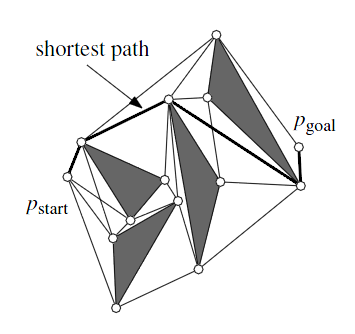
\includegraphics[scale = 0.4]{shortest}
	\end{figure} 
	Algorithm to calculate the visibility graph of $S^*$,
	
	\begin{algorithm}[H]
		
		\KwData{Set of Vertices Included in $S^*$ }
		\KwResult{Visibility Graph of $S^*$ }
		Initialize a graph $\gamma = (V,E)$ where $V$ is the set of al vertices of the polygons in $S$ and $E = \oslash$ 
		
		\For{<all vertices $v \subset V$>}
		{		
			W = VISIBLEVERTICES($v$,S)\;}
		
		
		\caption{VISIBILITYGRAPH($S^*$)}
	\end{algorithm}
	where $VISIBLEVERTICES(v,S)$ algorithm checks whether line segments drawn from $v$ to all vertices in $S$ is intersecting an interior area of any obstacle in the environment. With the help of this $VISIBILITYGRAPH$ algorithm $SHORTESTPATH$ algorithm can be defined as follows.
	
	\begin{algorithm}[H]
		
		\KwData{A set $S$ of disjoint polygonal obstacles, and two points $p_{start}$ and $p_{goal}$ in
			the free space.}
		\KwResult{The shortest collision-free path connecting $p_{start}$ and $p_{goal}$}
		1) Assign $\gamma$ = VISIBILITYGRAPH$(S^*)$
		
		2) Assign each arc $(v,w)$ in $\gamma_{vis}$ a weight, which is the Euclidian length of segment $vw$
		
		3) Use Dijkstra's algorithm to compute a shortest path between $p_{start}$ and $p_{goal}$ in $\gamma_{vis}$
		
		\caption{SHORTESTPATH}
	\end{algorithm}
	
	Dijkstra$'$s algorithm computes the shortest path between two nodes in
	graph with k arcs, each having a non-negative weight. It is a tree search algorithm and  used to calculate the shortest paths between nodes in a graphs, with the help of weighted edges between nodes. The time complexity of the original algorithm is $O(n^2)$ where $n$ is the number of the nodes in the graph. With the usage self balancing binary search tree, the algorithm requires $O(k+nlogn)$ time in the worst case. The algorithm for the Dijkstra's is given as follows:
	
		\begin{algorithm}[H]
		\KwData{$\gamma_{vis}$ , $source$\_$ node$ }
		\KwResult{Shortest Distance to Any Node from $source$\_$ node$ in $\gamma_{vis}$}
       	
		\For{<each vertex $v \subset \gamma_{vis}$>}
		{		
             Distance[v] := $\infty$ \;
			  Previous[v] := $undefined$ \;
		}
		Distance[$source$\_$ node$] :=0  \;
		Q:= The set of all vertices $v \subset \gamma_{vis}$ \;
		\While{<Q $\neq$ null>}
		{
			u:= Node in Q with smallest distance to $source$\_$ node$\;
			remove u from Q\;
			\For{<each neighbor v of u>}
			{
				alt:= Distance[u] + Cost Between u and v nodes\;
				\If{alt<Distance[v]}
				{
					Distance[v] :=alt\;
					Previous[v] :=u\;
					}
				}
			}
			return Previous[];
				
			\caption{DIJKSTRA'S ALGORITHM}
		\end{algorithm}
		In algorithm above $Distance[x]$ function call, calculates the total cost from the $source$\_$ node$ to the $x$ vertex, and $Previous[x]$ function call, returns the previous node in optimal path from $source$\_$ node$ .
	In our work, the weights of the edges in $\gamma_{vis}$ , are calculated with the Euler distance between nodes in the environment.  
			\subparagraph{Collaborative Decision Process of Final Goal States}\hspace{0pt} \\
	

	
In Section 2 and 3 possible routes and costs to the goal states are calculated with the help of Visibility Graphs and Dijkstra's algorithm  for each agent. It is obvious that each agent will try to choose a goal state with minimum cost according to its position and the orientation in the environment. But the cases in which two or more agents are willing to reach the same goal point must be handled by optimizing the overall utility of the swarm. To minimize to overall cost of whole swarm while achieving a formation shape, Hungarian algorithm which is a combinational optimization algorithm that solves this assignment problem is used. To implement this algorithm, a complete bipartite graph $G=(S,T,E)$ with $n \in S$ agents and $t \in T$ goal points is constructed.In this graph, each agent have a cost which is defined by the shortest path to the destination in the environment for different goal points. 
	\begin{figure}[H]
		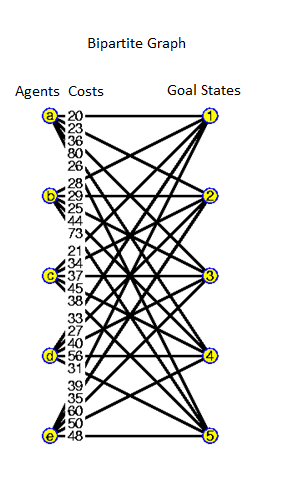
\includegraphics[width=.4\textwidth,center]{bipartite}
		\caption{Sample Bipartite Graph Used in Assignment Problem}
	\end{figure}

	A cost matrix  $C$ is defined to implement the Hungarian algorithm .  The dimensions of the cost matrix is $nxm$ in which each element represents the cost of assigning the goal state $m$ to the agent $n$.  Since we have equal number of agents and goal states, the cost matrix will be a square matrix with $nxn$ or $mxm$.  The algorithm for the assignment process as follows:
	
	
	
	\begin{algorithm}[H]
		\KwData{Cost Matrix , $C$ }
		\KwResult{Assignment Array of Agents to Goal States}
	
	     Label1  \;
	     \For{Each Row, $R$, in $C$ }{
	     	Find the smallest element and subtract it from every element
	     	}
	   Label 2  \; 
	   \If{A Column,$K$, contains more than one zero}
	   {Repeat Label1 for each column, $K$}
   
      Label 3  \; 
      Select element in columns for which a distinct minimum weight has been determined and add to solution
     
     Label 4 \;
     If it is not possible to reach the full solution, flag rows without solutions. Flag all columns in flagged rows that contain a zero. Flag all rows with a previously determined solution in previously flagged columns.
     
     Label 5 \;
     From elements remaining in flagged rows and unflagged rows, determine the element which has smallest value and assign this value to $\gamma$. Subtract $\gamma$  from every unflagged element and add  $\gamma$ to every element that has been flagged twice.
     
     Label6 \;
     Goto Label3 until full solution has been achieved.
     
     		\caption{HUNGARIAN ALGORITHM}
		\end{algorithm}
	
	\paragraph{Control System Design for Individual Agents}\hspace{0pt} \\
Shape partitioning methods will provide the goal states for a desired formation shape and agents will be assigned to those goal states to minimize the overall energy consumption of the swarm. A control system which will guide the agents to reach these goal states must be designed for each agent individually. Since the environment is dynamically changing with lots of  mobile agents, it is very probable to have different assignments to these goal states at each iteration of formation control. On the other hand, the collision with the obstacles and the other agents at the environment must be prevented due the requirements presented in Section-xx. The control system must react to these dynamic requests. A velocity controller with a large bandwith is designed at the inner loop of the control system and the outer loop is composed with a velocity setpoint generator. The block diagram for the proposed controller structure is presented in Figure -xx.


			\begin{figure}[H]
				\caption{General Scheme of the Contol System}
				\centering
				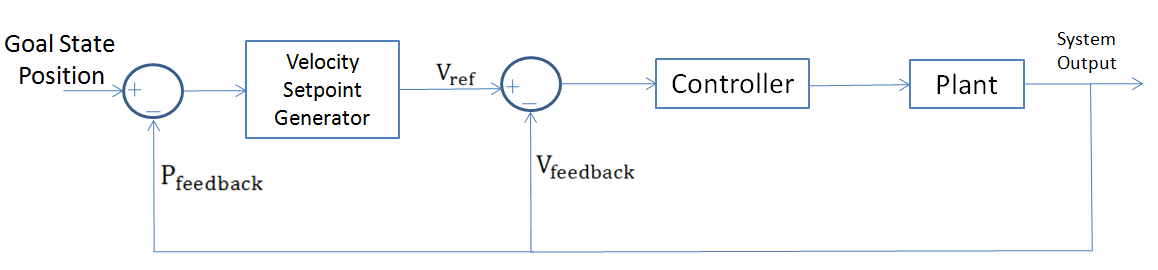
\includegraphics[scale = 0.45]{controller}
			\end{figure}


Velocity setpoint generator provides instant setpoints for the inner loop based on the current position of the agent and the desired goal state position.  This loop calculates the amplitude of the velocity setpoint proportinal with the euclidian distance of agent to the desired goal state. The direction of this velocity setpoint vector has a bearing angle of the line segment drawn from the agent to the goal state. This generator saturates the amplitude of the setpoint vector with 0.5 [m/sec] to prevent the agents' travelling in the environment so fast. 
	\begin{figure}[H]
		\caption{Velocity Setpoint Generation}
		\centering
		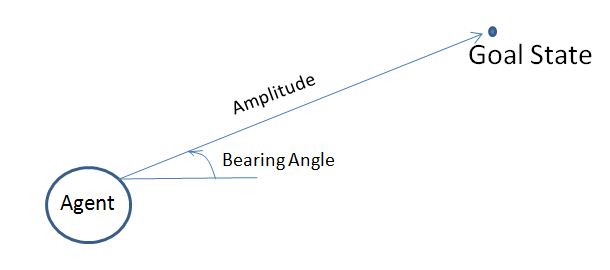
\includegraphics[scale = 0.50]{bearing}
	\end{figure}



The inner loop tis designed to track the velocity setpoint provided by the generator and it has a state feedback structure. The gains for the feedback states are calculated with an LQR controller. A simple mass, damper type second order linear system is used to provide a model for the controller. The translational friction force is assumed to be linear with the velocity of each agent. Different mass and friction coefficients for heterogenous mobile robots are used in control system design. To track the desired velocity setpoint, the model of the system is augmented with an artificial error state,

\begin{equation}
\begin{bmatrix}
\dot{v} \\ \dot{e}
\end{bmatrix}
=
\begin{bmatrix}
-b/m & 0 \\
1 & 0
\end{bmatrix}
\begin{bmatrix}
v \\ e
\end{bmatrix}
+ \begin{bmatrix}
1/m \\ 0
\end{bmatrix}
F_{net} \hspace{0.5cm} and
\hspace{0.5cm}
y = \begin{bmatrix}
1 & 0
\end{bmatrix}
\begin{bmatrix}
v \\ e
\end{bmatrix}
\end{equation}

where $b$ is the linear friction force coefficient and $m$ is the mass, $v$  is the linear velocity of the agent and $e$ is the augmented error state which is the integral of the velocity state. Here the $v$ state is the stabilizing part of the controller and the $e$ error state is the tracker part of the controller. The state feedback gain, $K$, which minimizes the quadratic cost function of
\begin{equation}
 J = \int_{t_o}^{t_1}(x^TQx + u^TRu) dt
\end{equation}
is calculated with help of $'lqr'$ function of MATLAB for the given system in $106 - degisebilir$ with the gain matrices of 

\begin{equation}
 Q = \begin{bmatrix}
q_1 & 0 \\ 0 & q_2
 \end{bmatrix}
 \hspace{0.3cm} and
\hspace{0.3cm}
 R = r_1
\end{equation}
the parameters for the controller design are determined with the approach presented below,
\begin{equation}
q_1 = \frac{1}{t_1 (x_{1max})^2}; \hspace{0.1cm}
q_2 = \frac{1}{t_2 (x_{2max})^2}; \hspace{0.1cm} and \hspace{0.1cm}
r_1 = \frac{1}{ (u_{1max})^2}; \hspace{0.1cm}
\end{equation}
Here $t_i$  is the desired settling time for $x_i$ which is determined as 1.5 seconds for the velocity and 0.001 seconds for the integral state. The statement of $x_{imax}$ represents the expected maximum value of the state $i$ , which is defined 1 [m/sec] for the velocity state and 4 [m] for the error state. $u{1max}$ represent the maximum allowable input signal which is defined 3 [N]. The structure of the inner loop is illustrated in Figure-xx
	\begin{figure}[H]
		\caption{Inner Loop Structure}
		\centering
		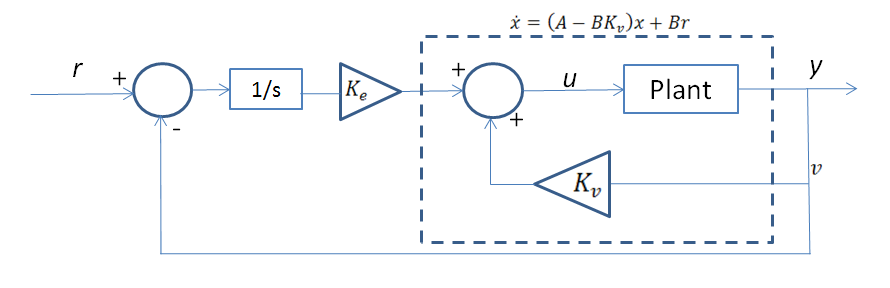
\includegraphics[scale = 0.50]{inner_loop}
	\end{figure}



The error between the reference and the velocity feedback is integrated and multiplied with the error gain, and the velocity state is multiplied with the velocity gain. These two components generate the total control input of the system.  

	\begin{figure}[H]
		\caption{Step Response of the Closed Loop}
		\centering
		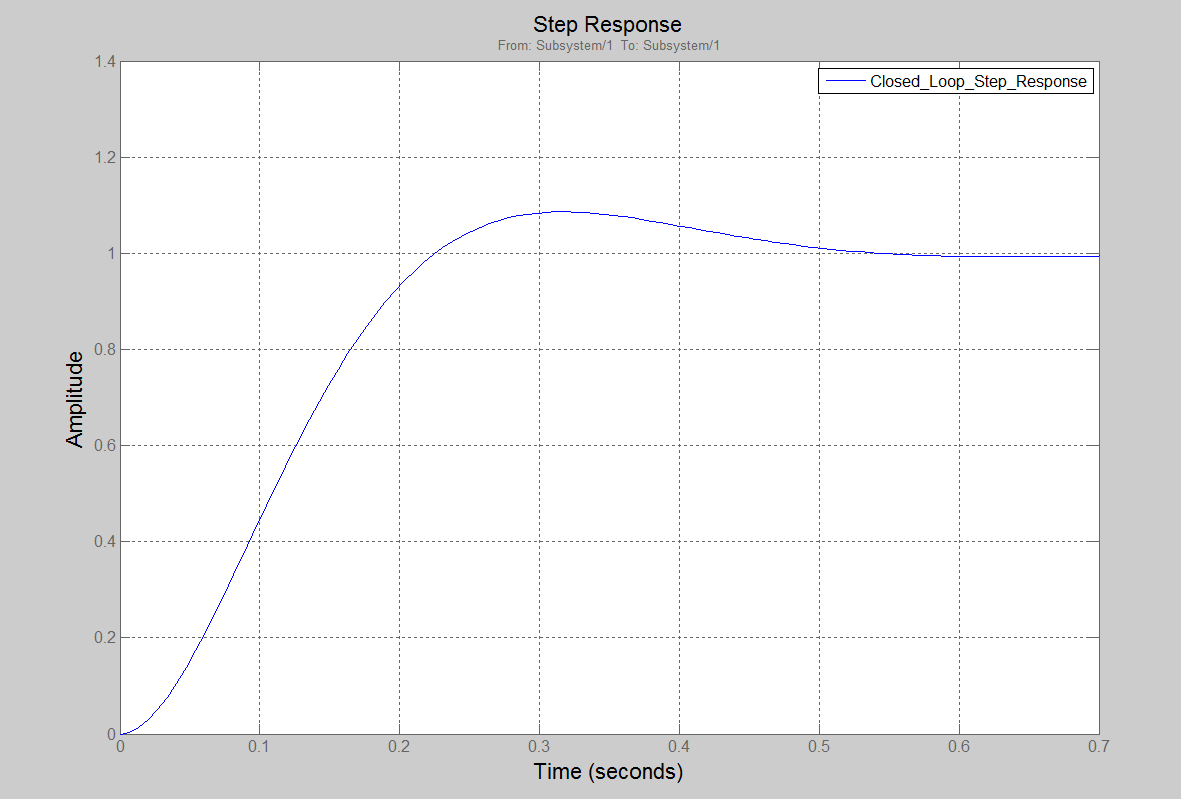
\includegraphics[scale = 0.50]{step_resp}
	\end{figure}

According to the Figure -xx, the settling time for the inner loop is around 0.5 seconds for a step input. This response characteristics is important since the system cannot react to the setpoints changing faster than 0.5 seconds, so the formation control loops in which the new goal state assignments are handled must be executed with 2Hz frequency. 

